%xelatex
\documentclass{article}

%\usepackage[T2A]{fontenc}
\usepackage[english,ukrainian]{babel}
\usepackage{fontspec}
\setmainfont{Nimbus Roman}
\usepackage{graphicx}
\usepackage[a4paper,margin=0.5in]{geometry}
\usepackage{amsmath}
\begin{document}

\pagestyle{empty}
\begin{center}

	{\fontsize{14}{24}\selectfont МІНІСТЕРСТВО ОСВІТИ І НАУКИ УКРАЇНИ

	НАЦІОНАЛЬНИЙ УНІВЕРСИТЕТ «ЛЬВІВСЬКА ПОЛІТЕХНІКА»

	Інститут комп'ютерних наук та інформаційних технологій

	Кафедра ОМП

	}

	\vspace{90.4pt} %120.4+16.1
	\begin{figure}[h]
		\centering
		
\includegraphics[width=6.5cm,keepaspectratio]{../../lpnu.png}
	\end{figure}

	{\fontsize{18}{29}\selectfont{Звіт}

	{до розрахункової роботи №1}

	{З дисципліни}

	{``Алгебра та геометрія''}

	{Варіант 12}

	}
\end{center}

\vspace{12.1pt} %30.1pt
	{\fontsize{14}{22.4}\selectfont
\begin{flushright}
	\textit{Виконав:}

	\textit{студент групи ПП-14}

	\textit{Мілюхін Олександр}

	\textit{Прийняв:}

	\textit{Баранецький Я. О.}
\end{flushright}
\vspace{37.4pt} %100.4
\begin{center}
\textit{Львів-2022}
\vspace{37.4pt} %100.4
\end{center}
	}
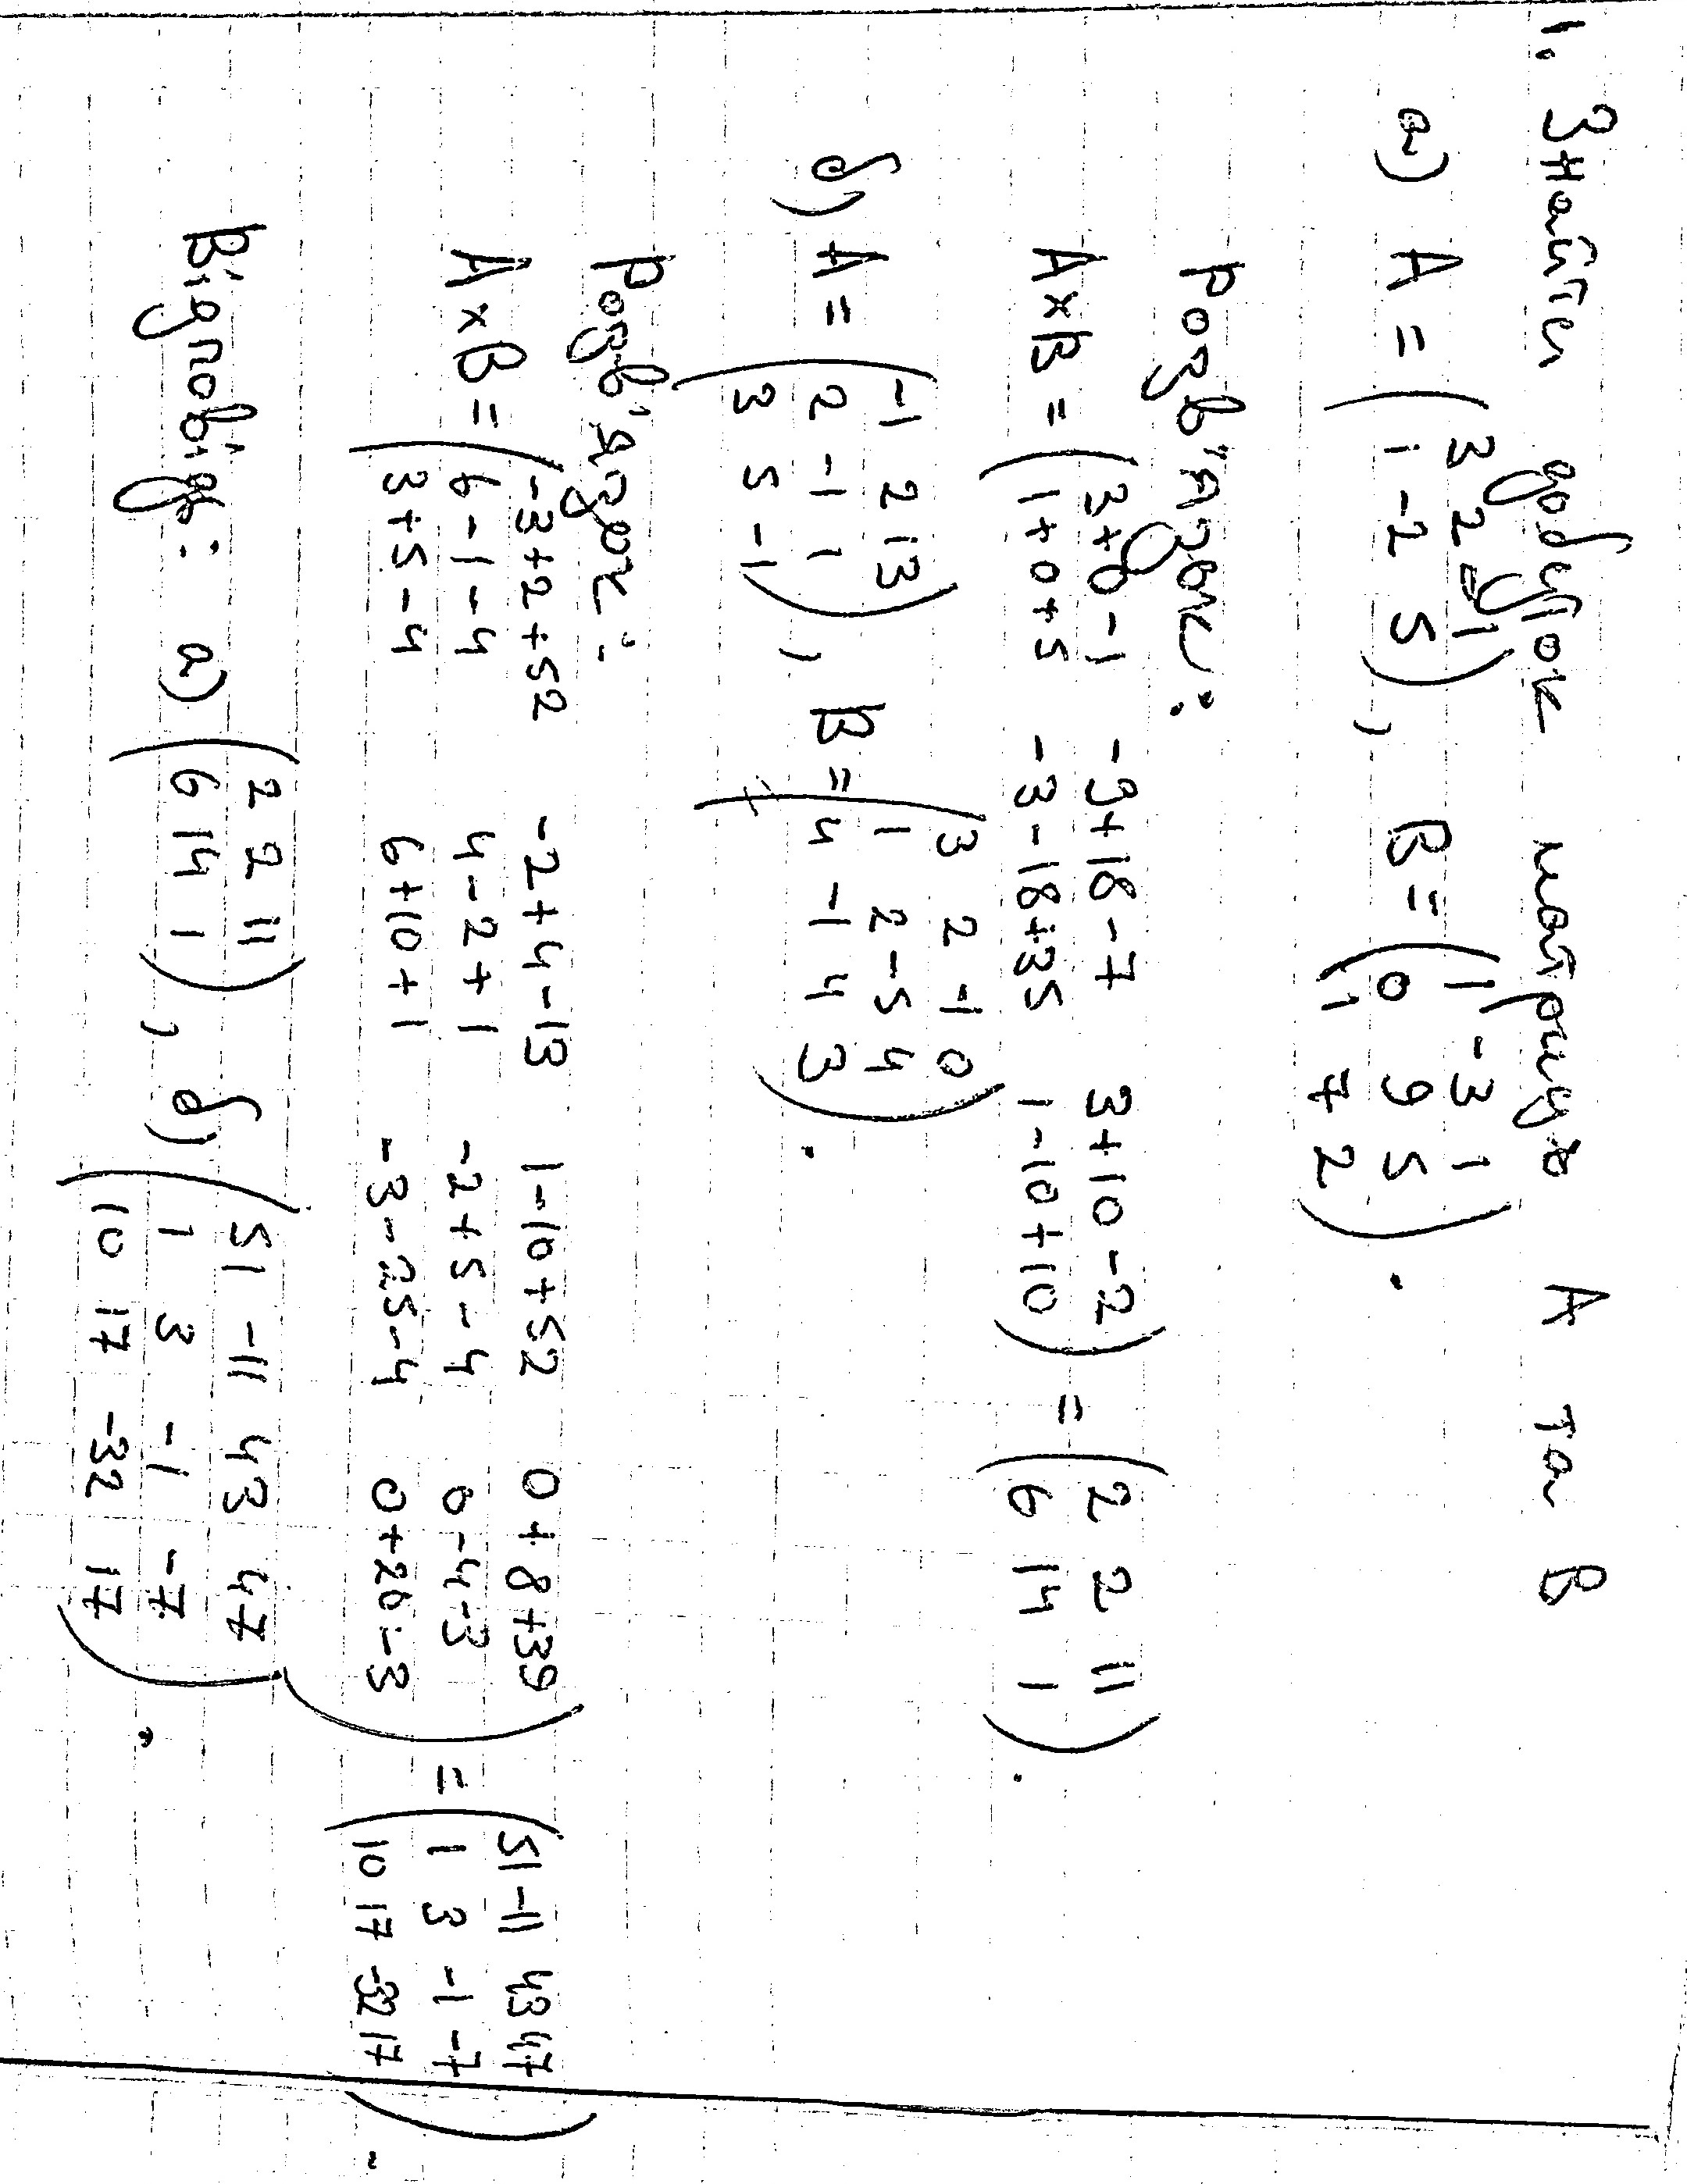
\includegraphics[width=12cm,angle=90]{ons/1.jpg}\\
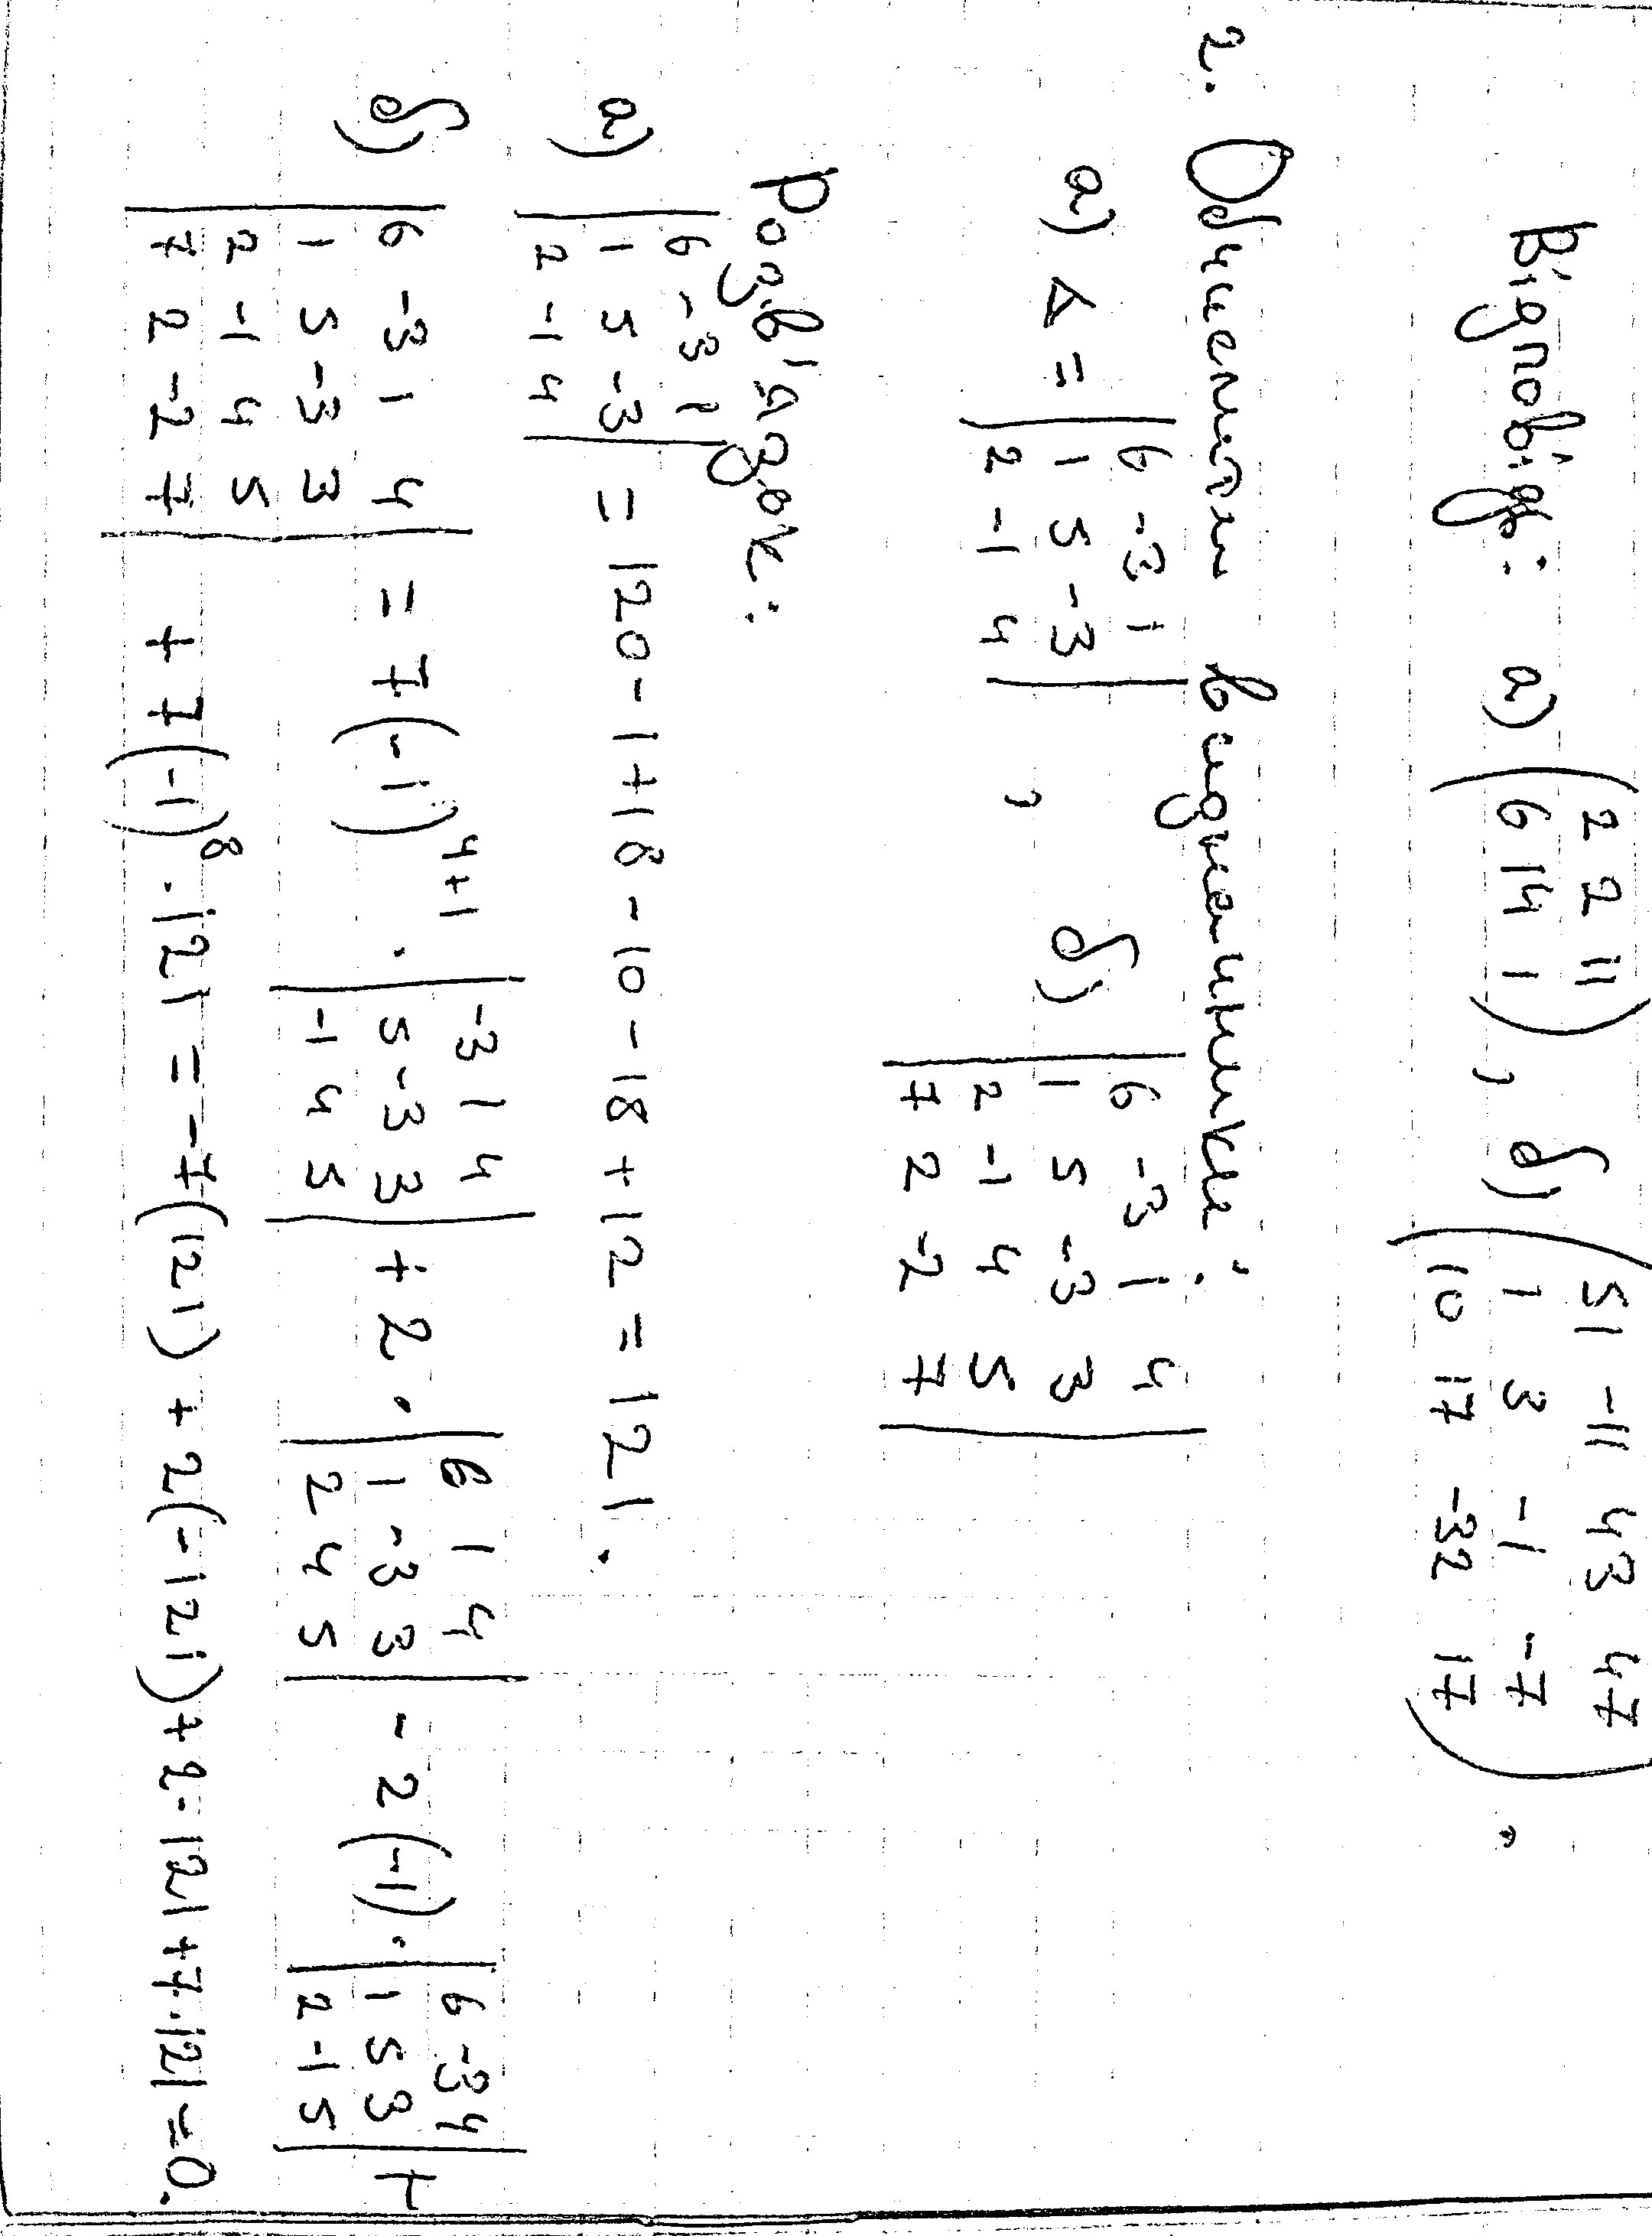
\includegraphics[width=12cm,angle=90]{ons/2.jpg}\\
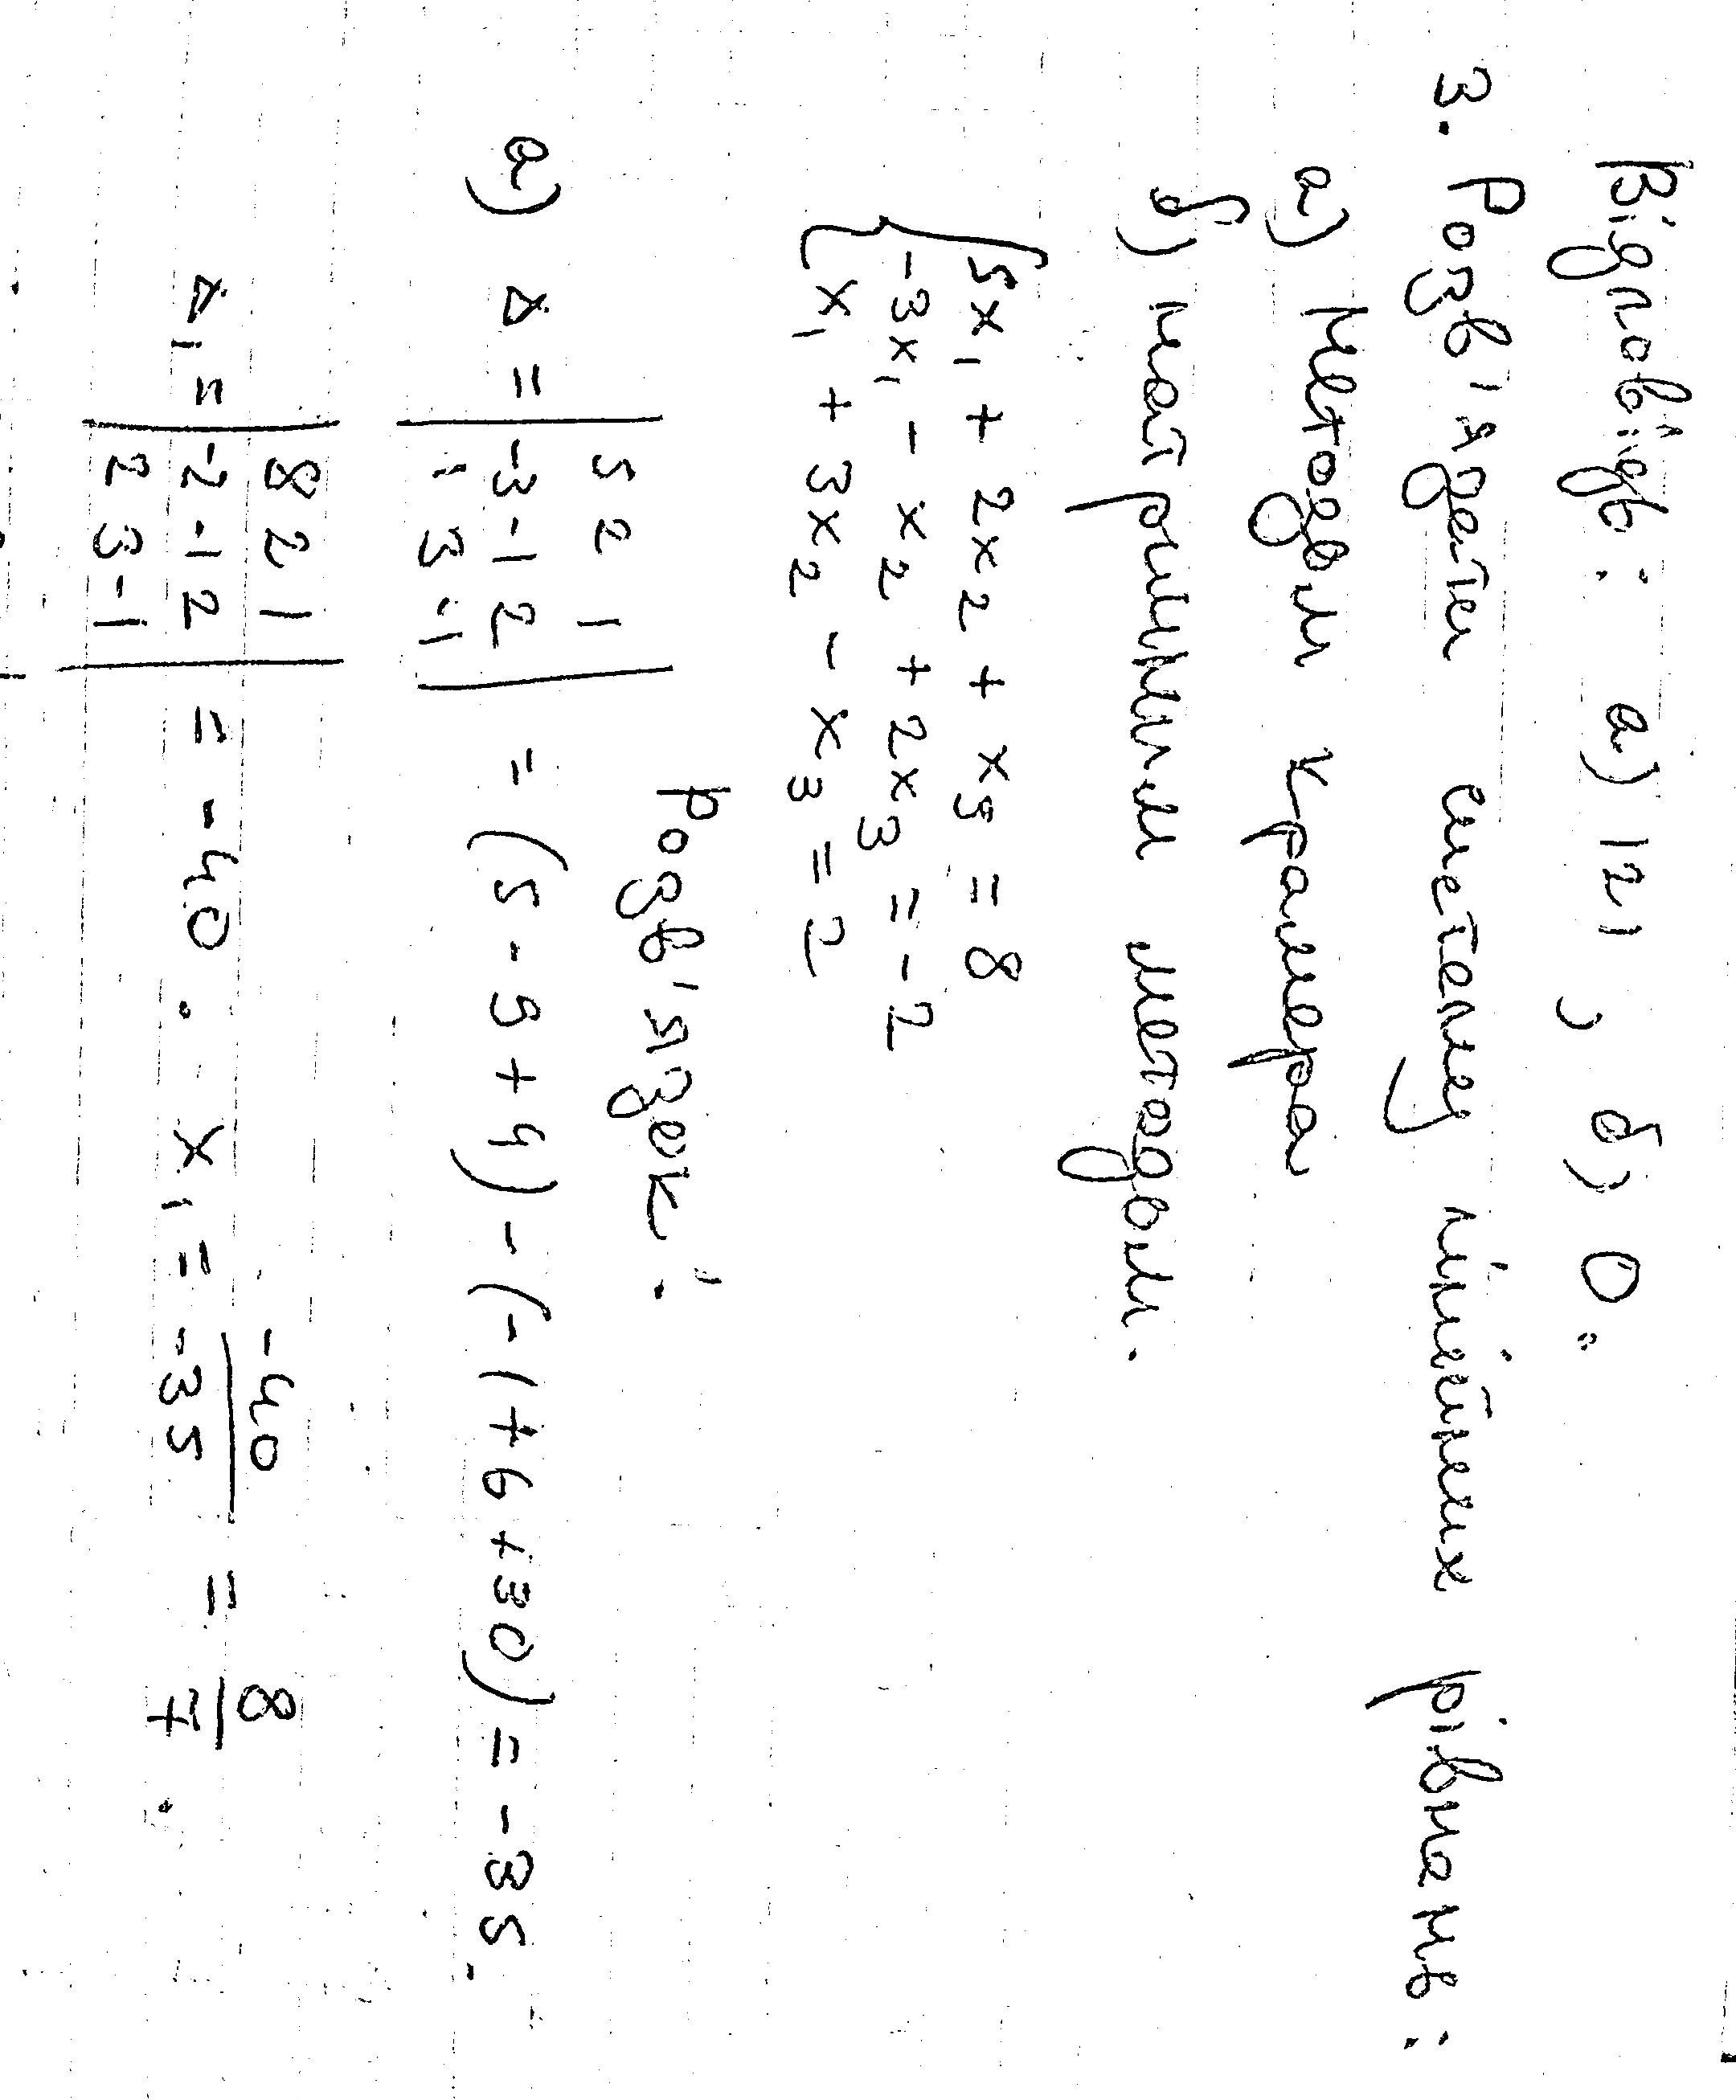
\includegraphics[width=12cm,angle=90]{ons/3.jpg}\\
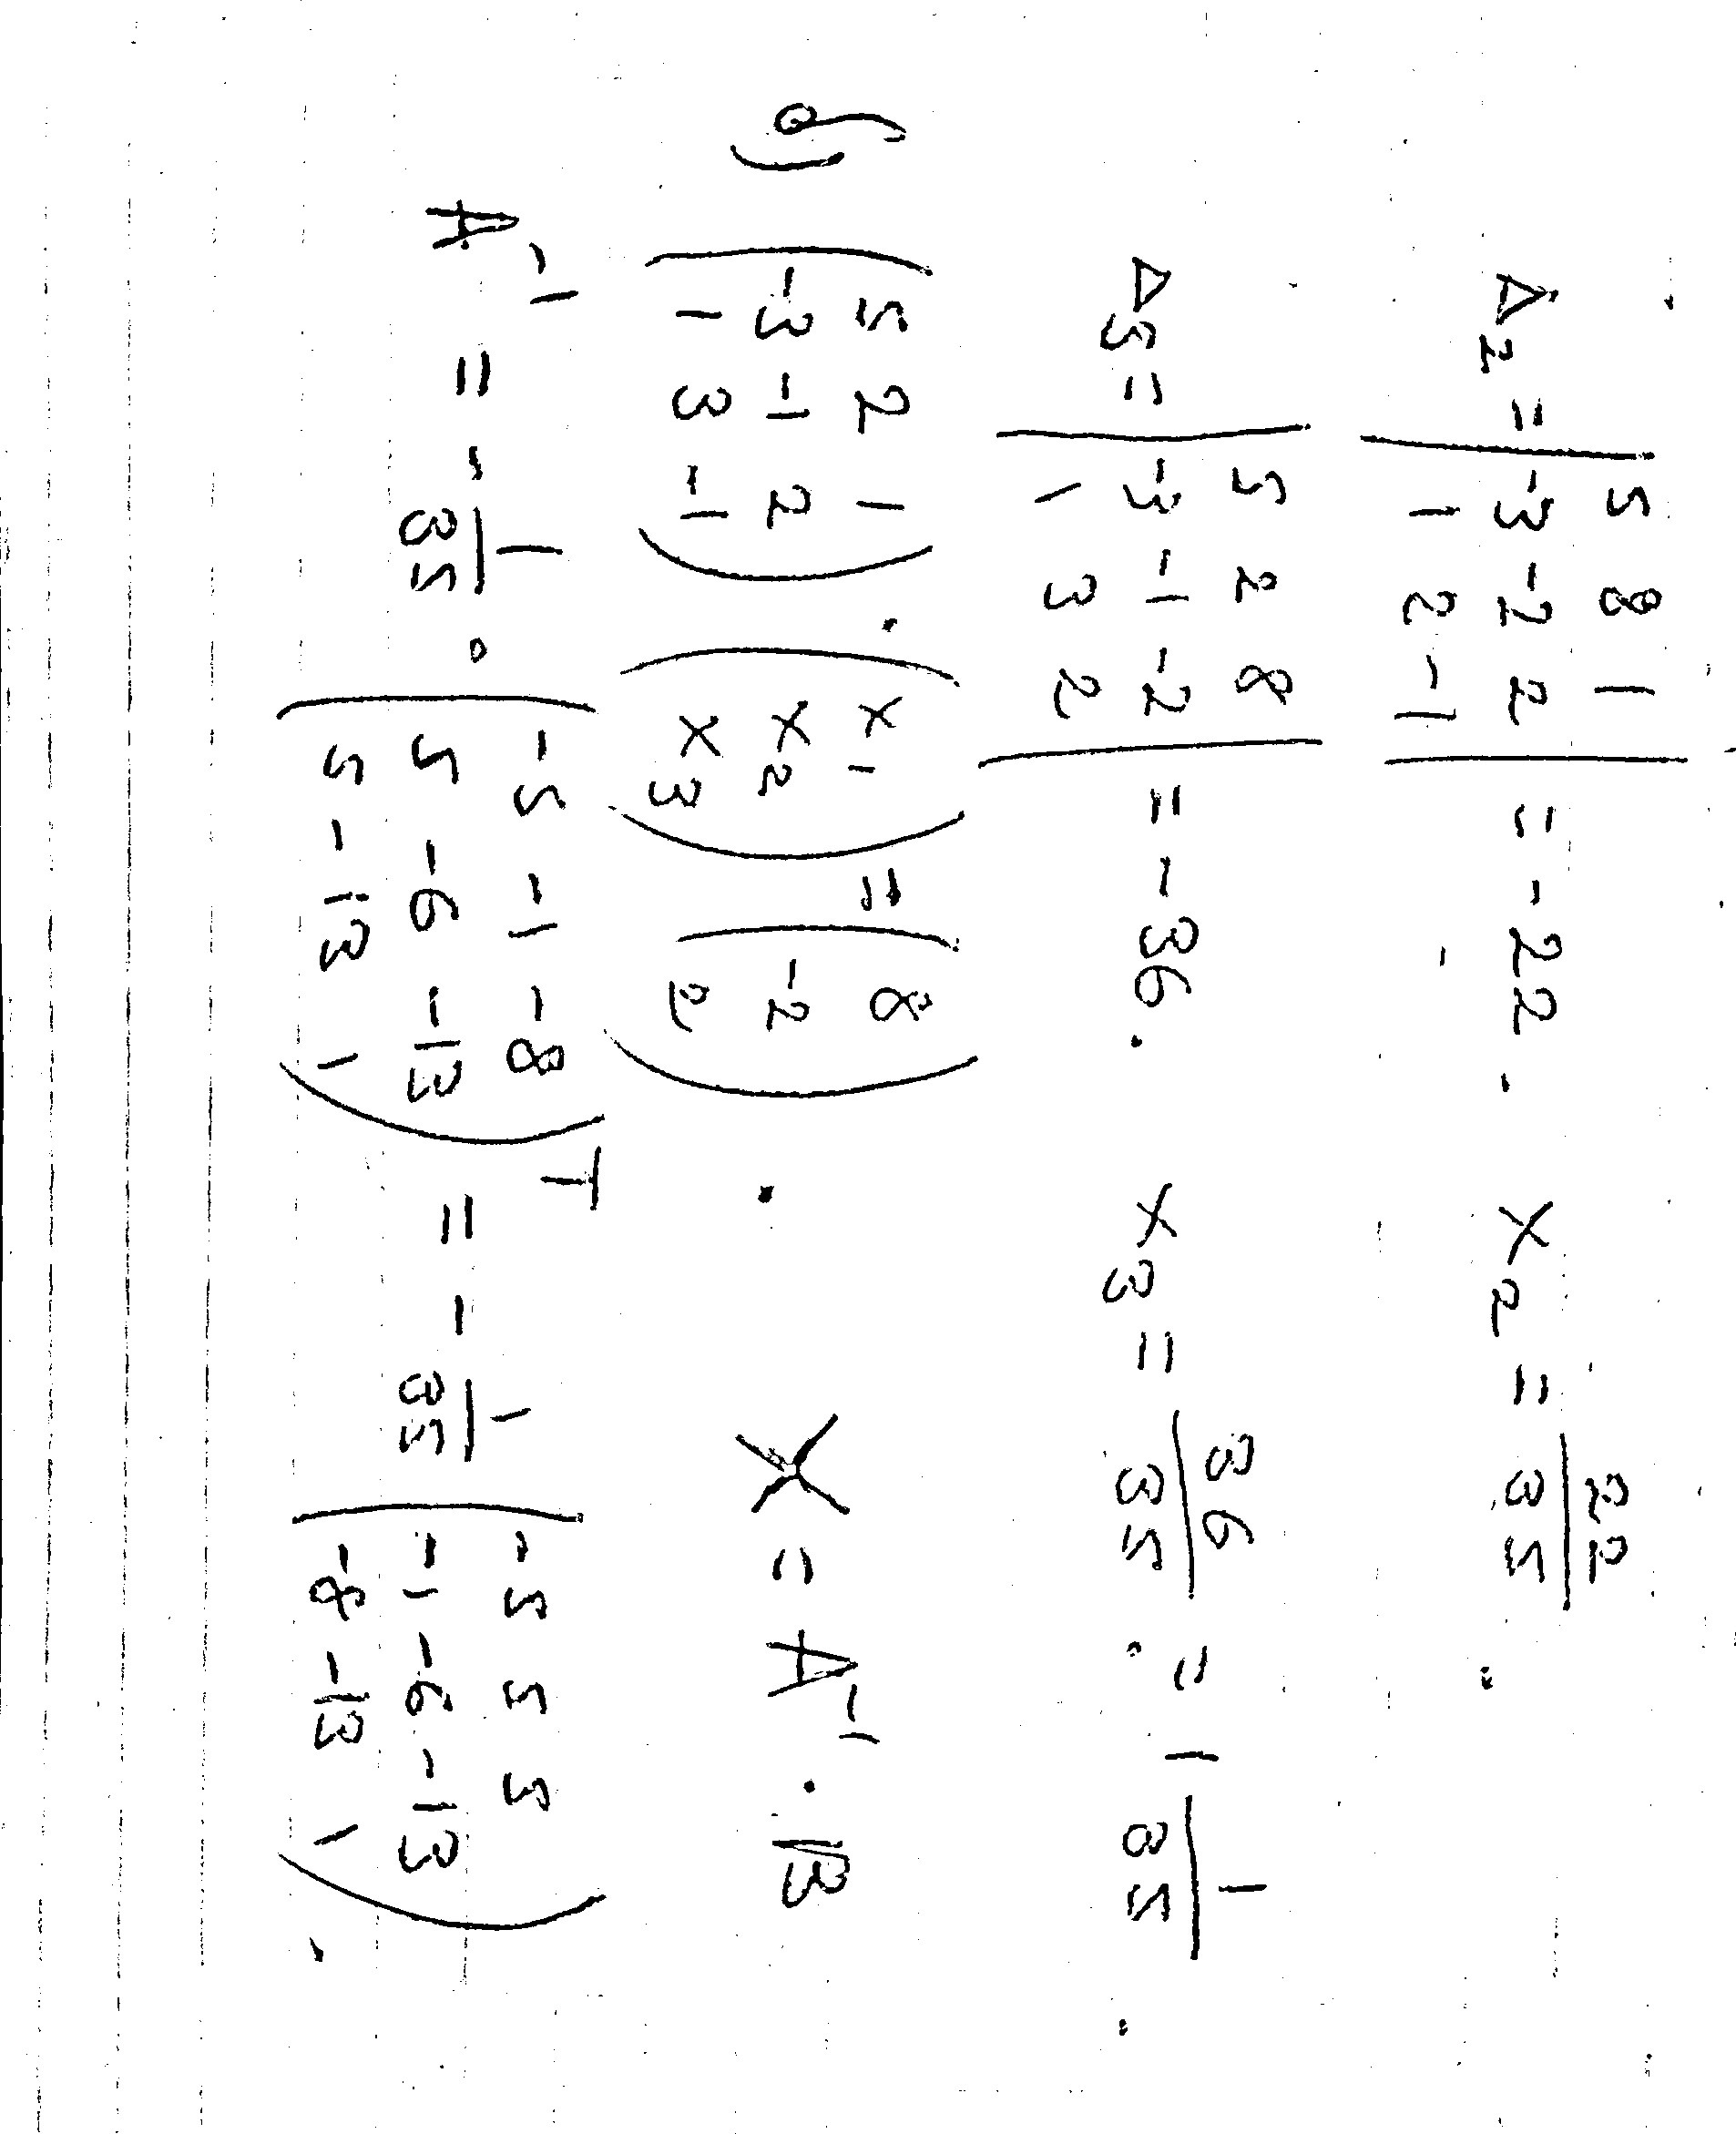
\includegraphics[width=12cm,angle=90]{ons/4.jpg}\\
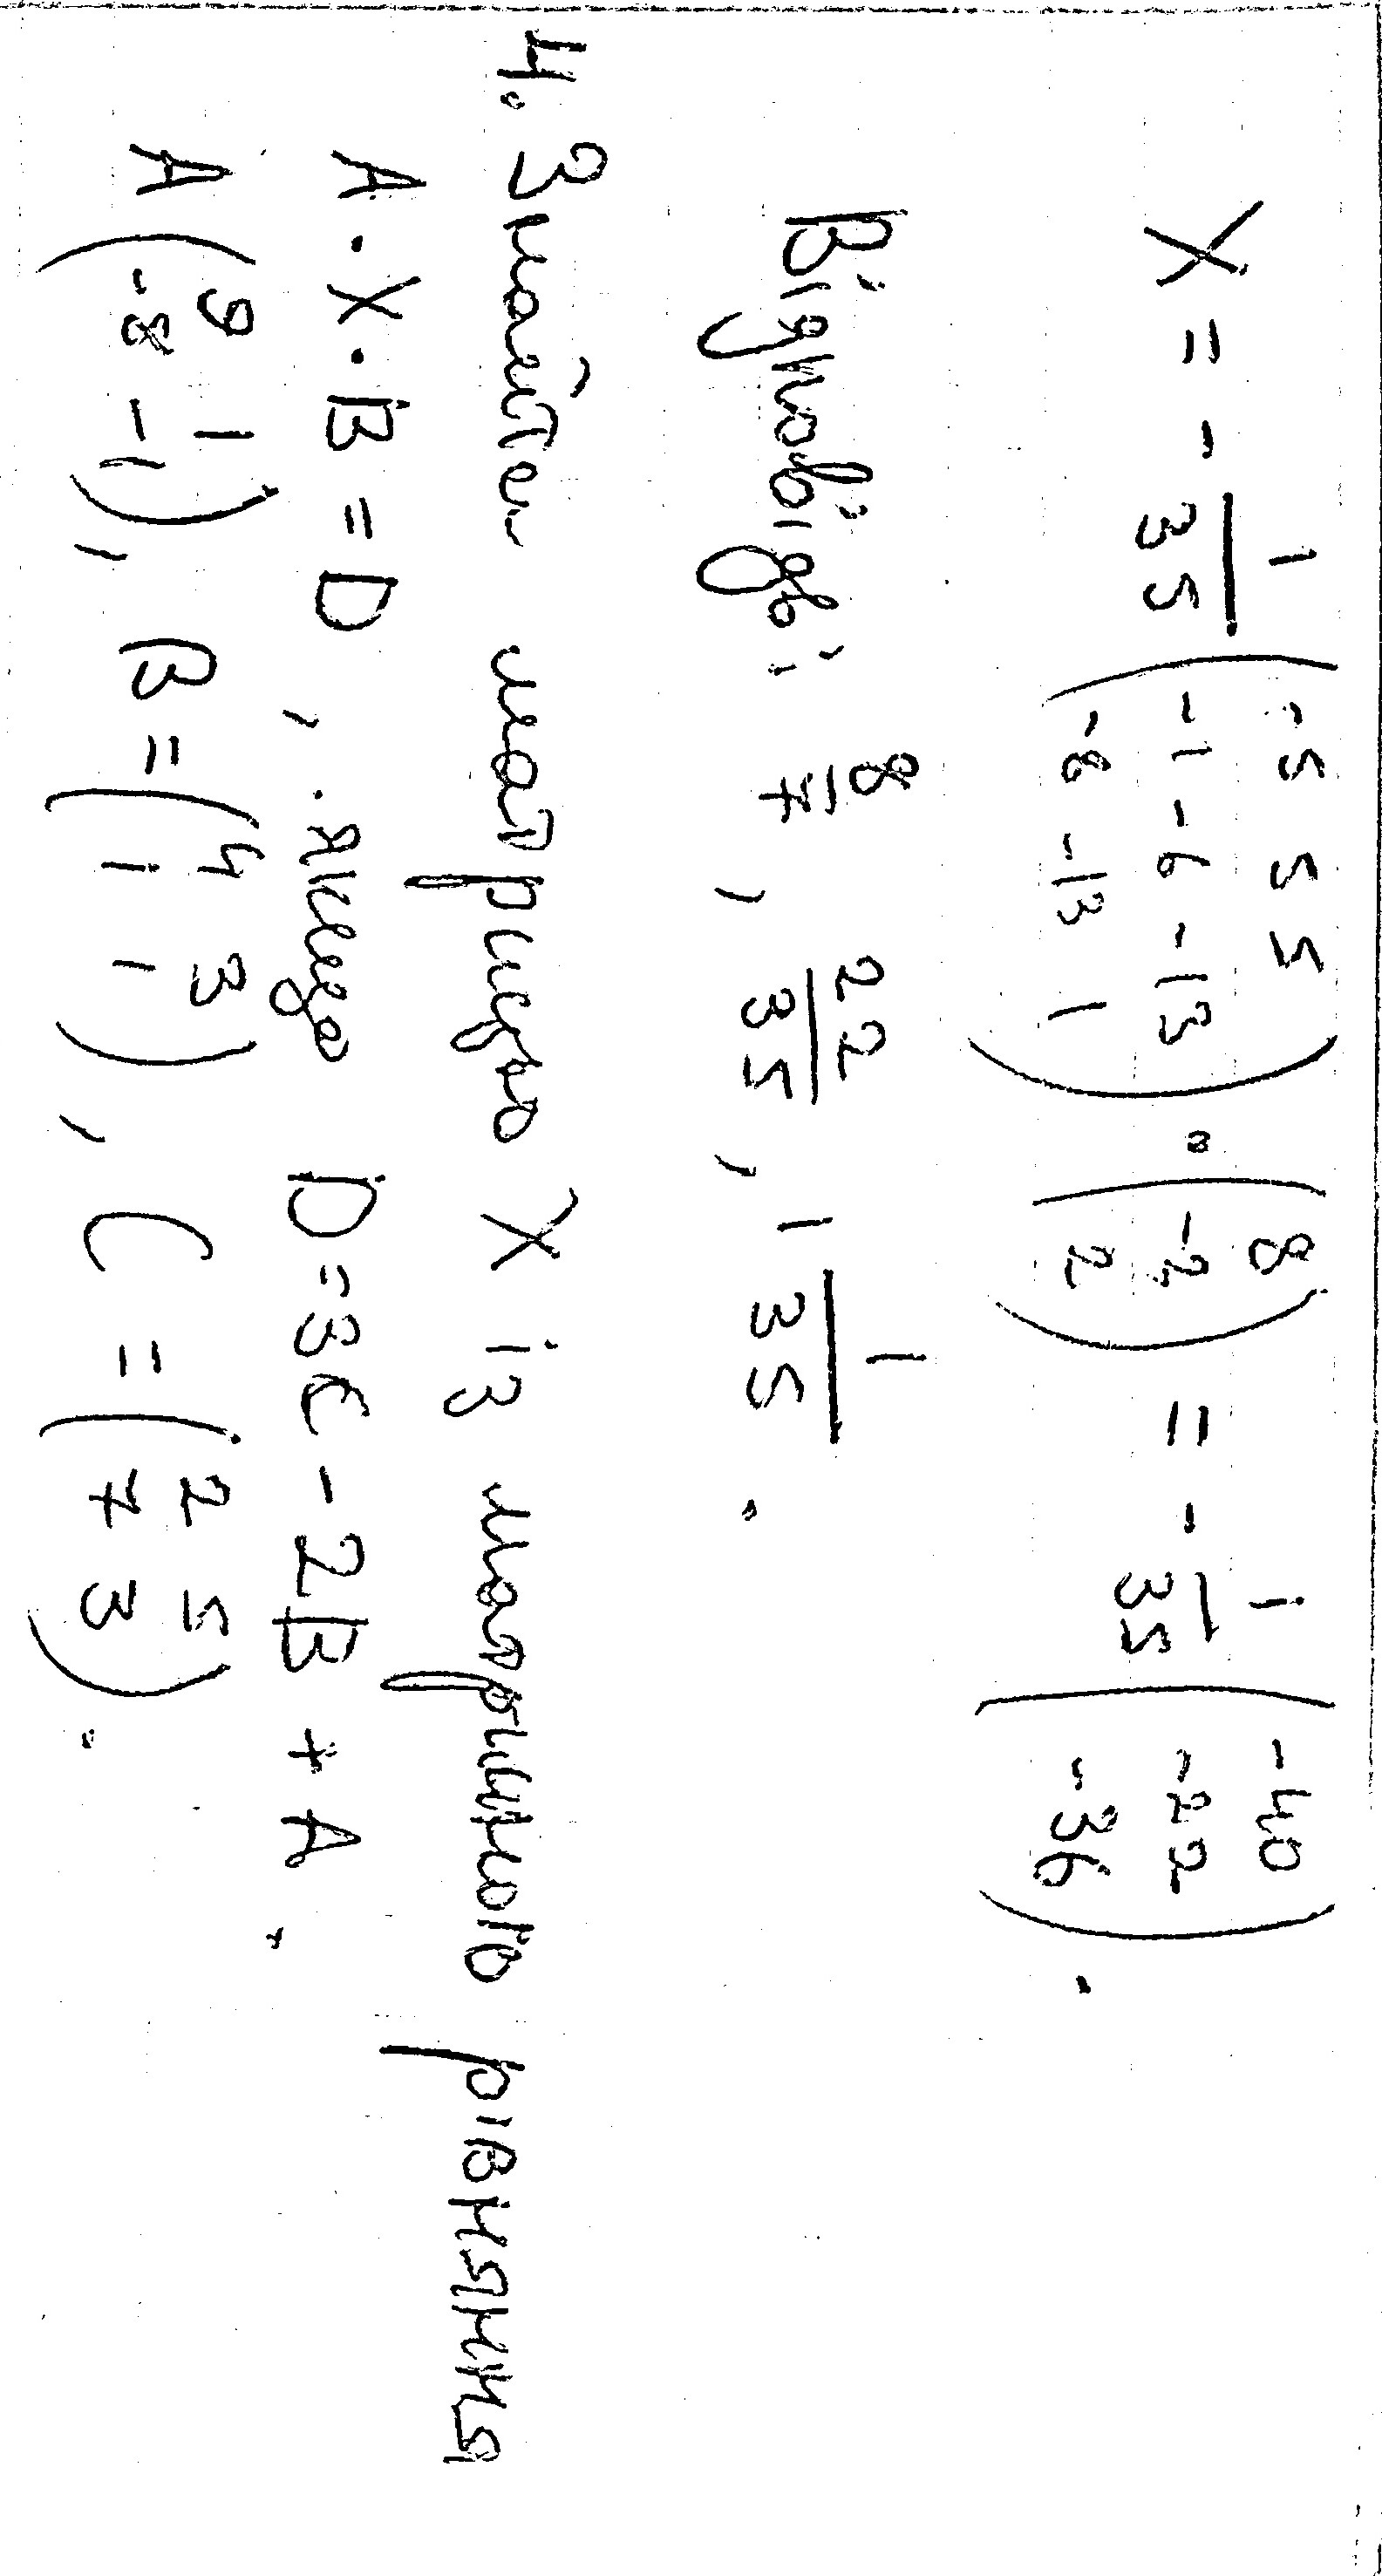
\includegraphics[width=10cm,angle=90]{ons/5.jpg}\\
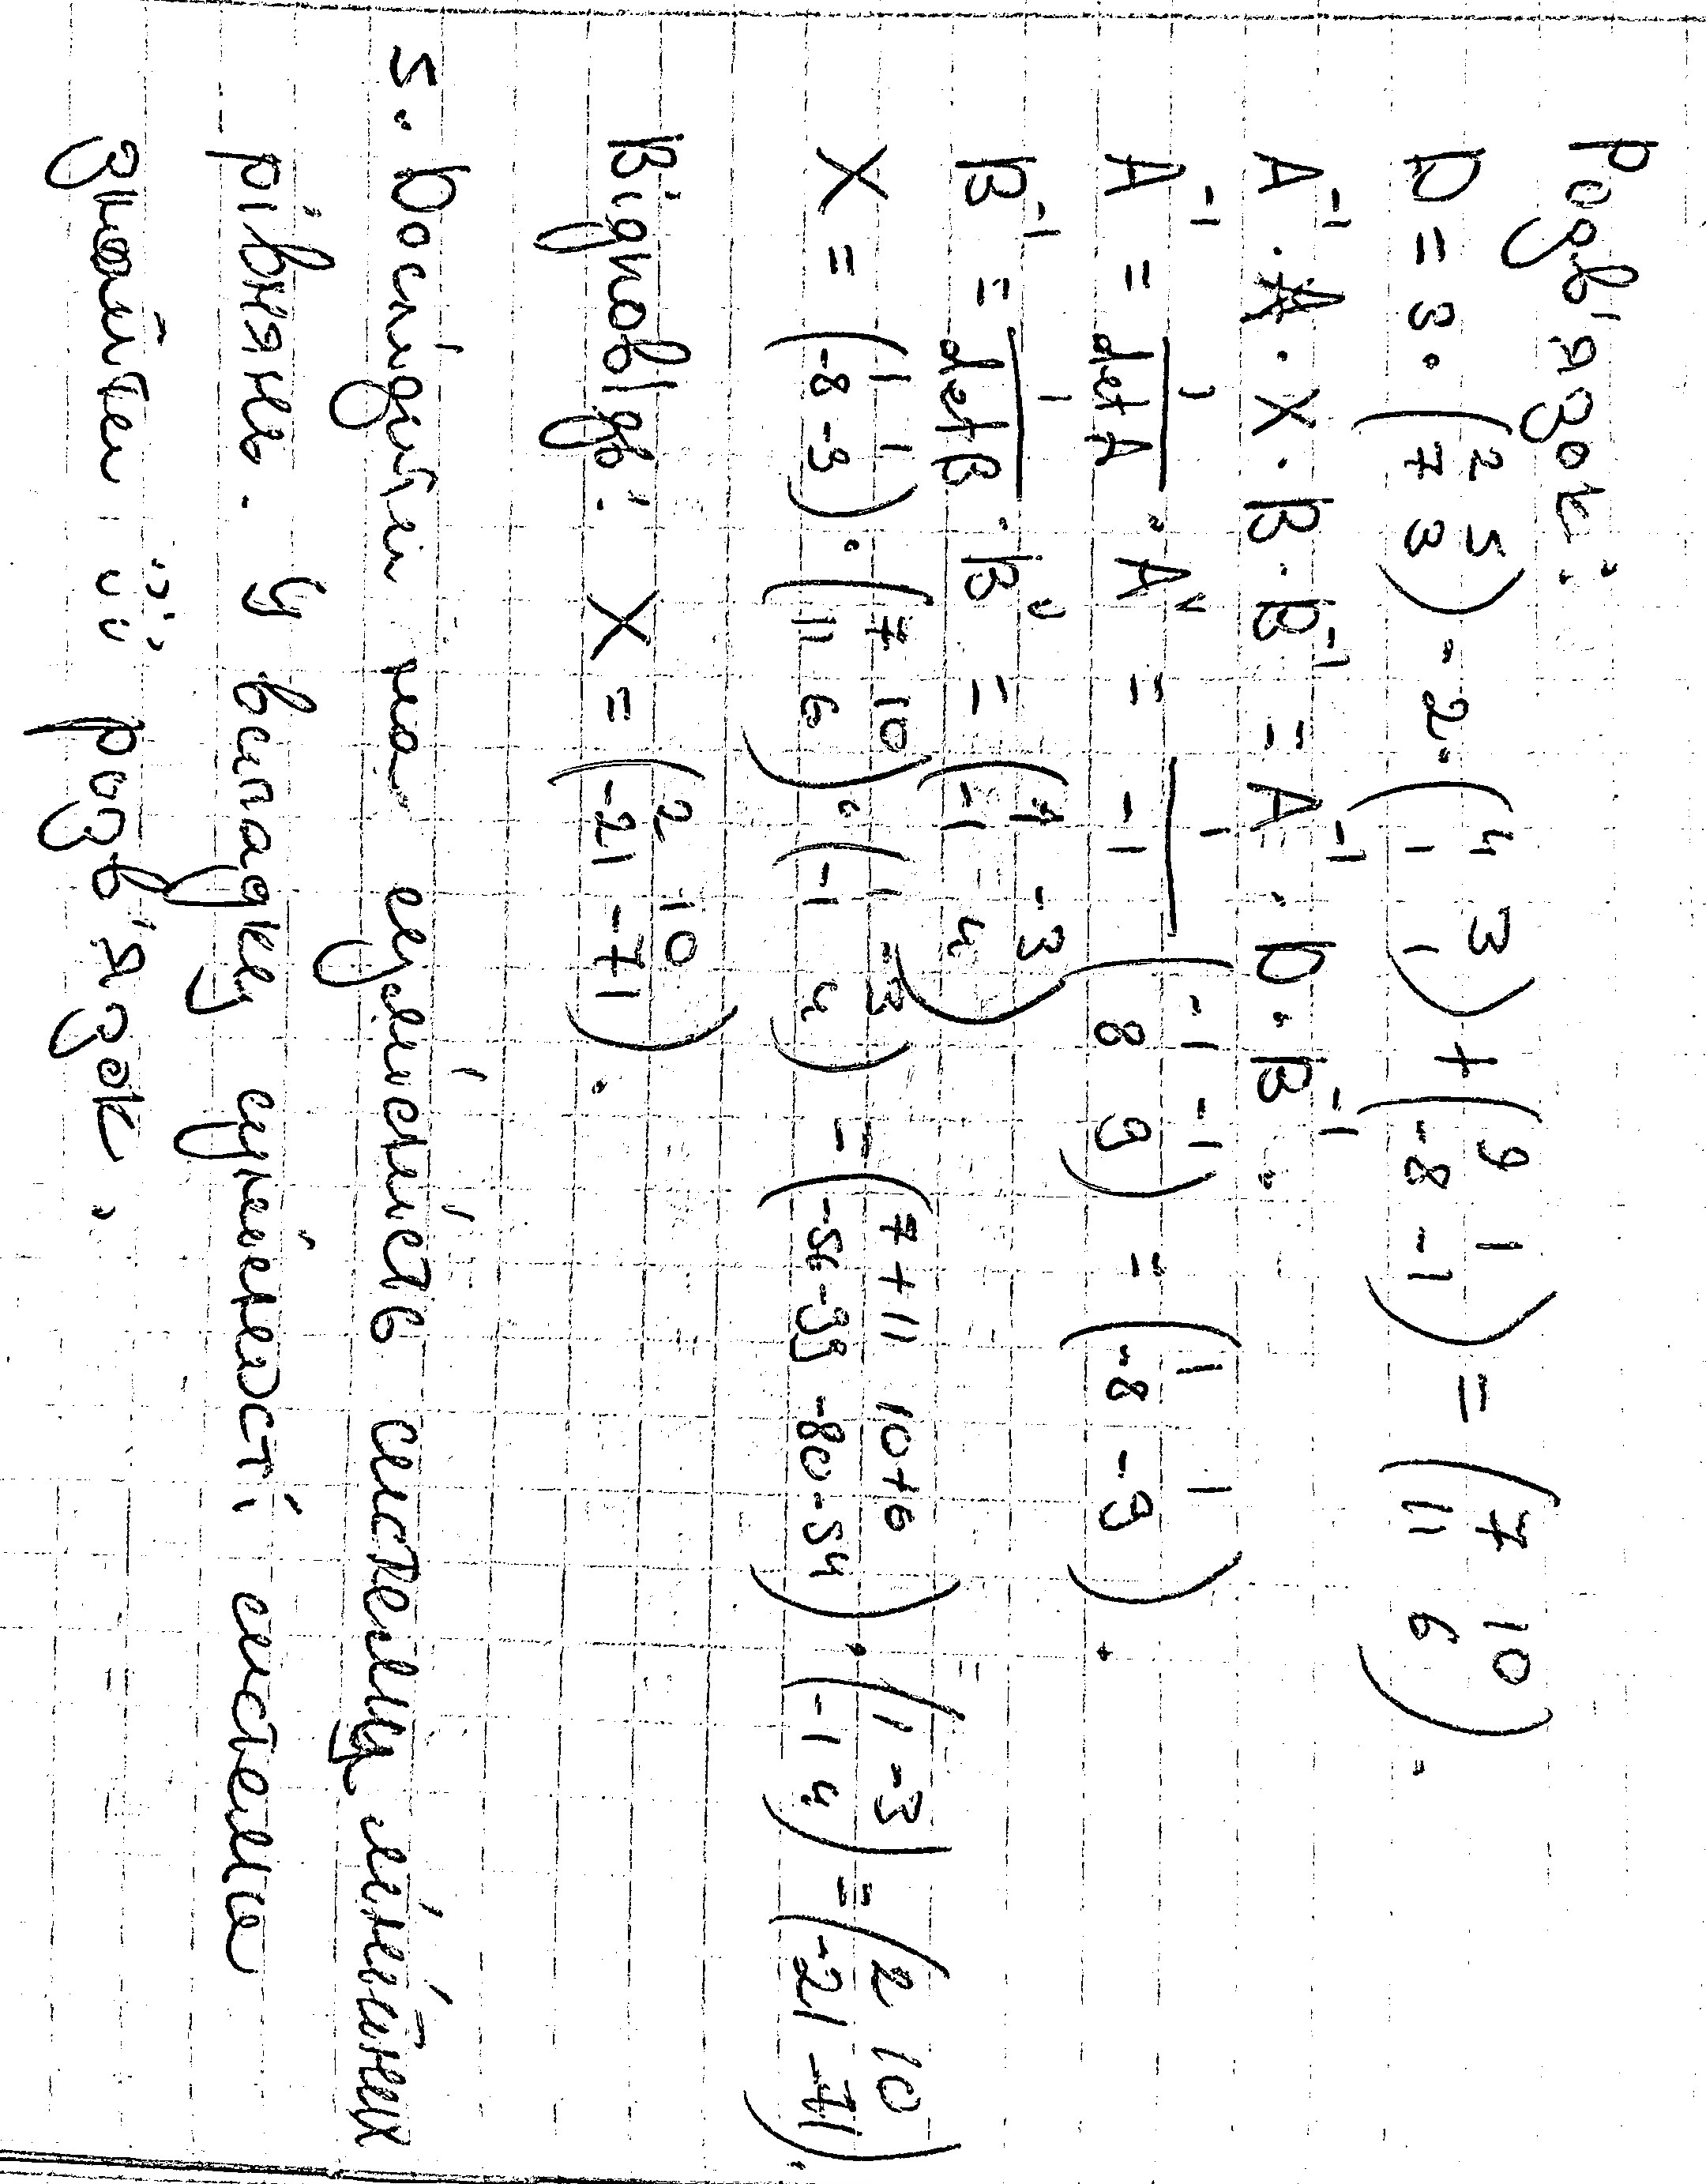
\includegraphics[width=14cm,angle=90]{ons/6.jpg}\\
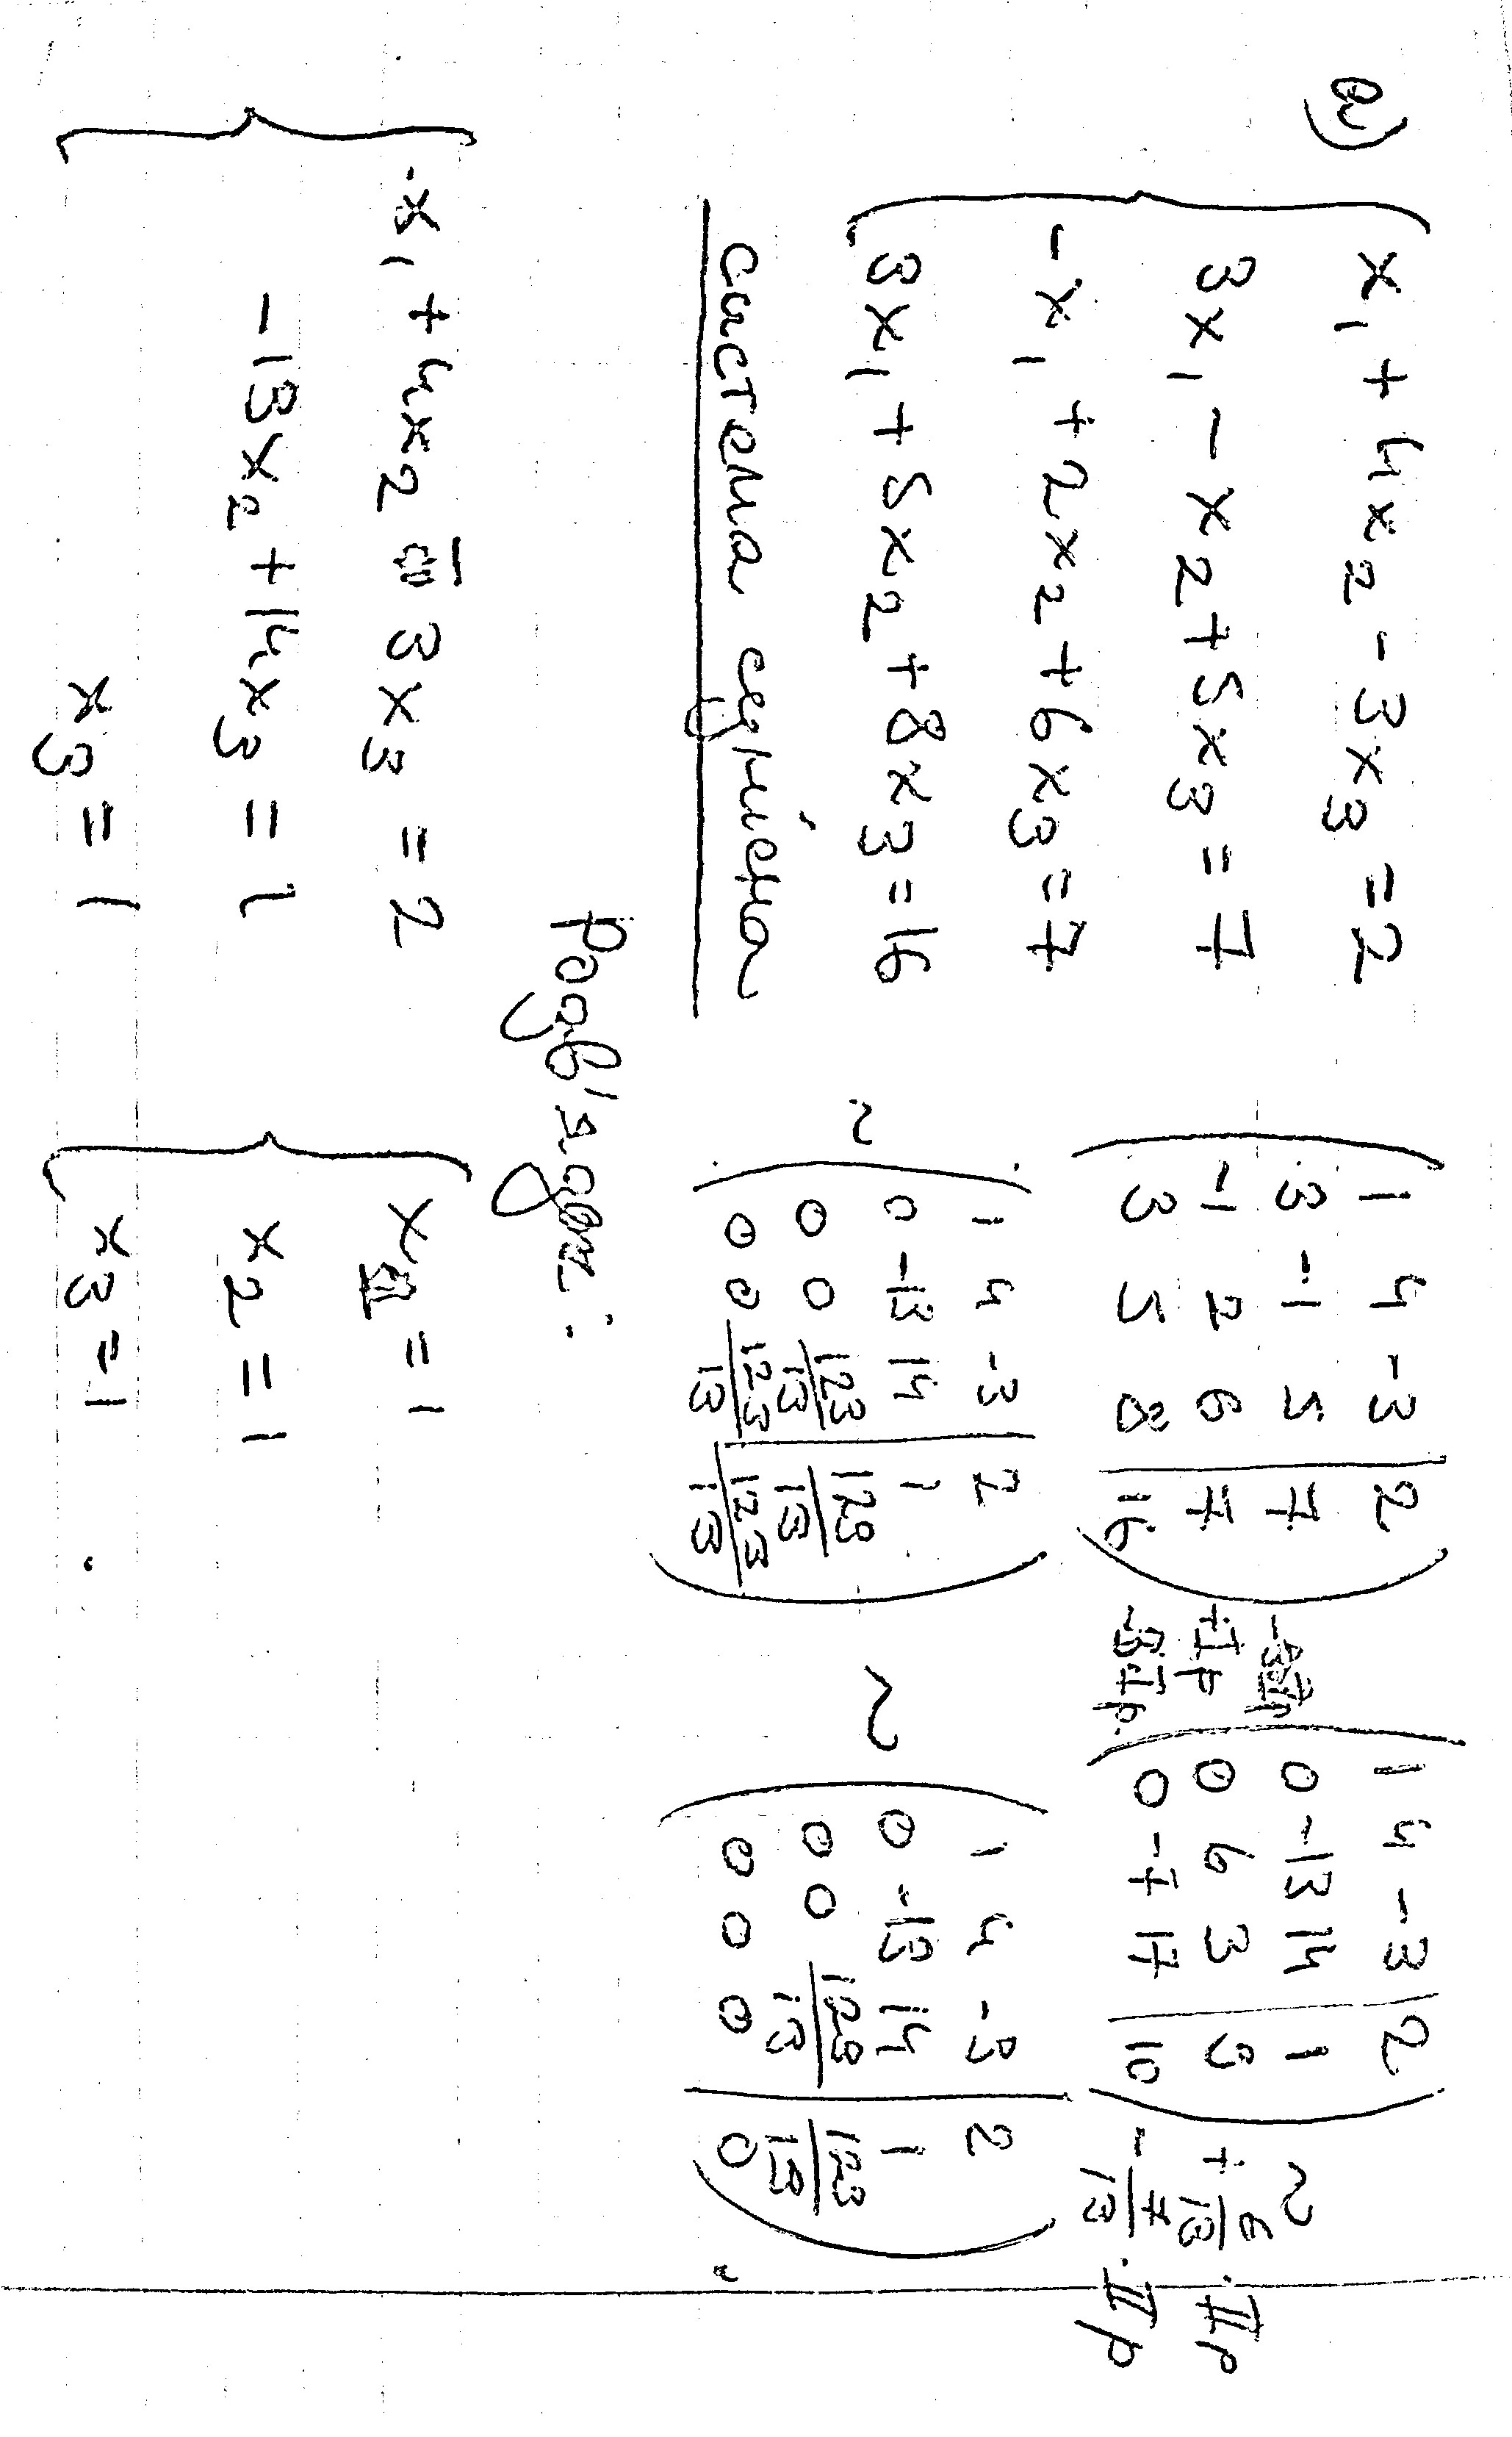
\includegraphics[width=11cm,angle=90]{ons/7.jpg}\\
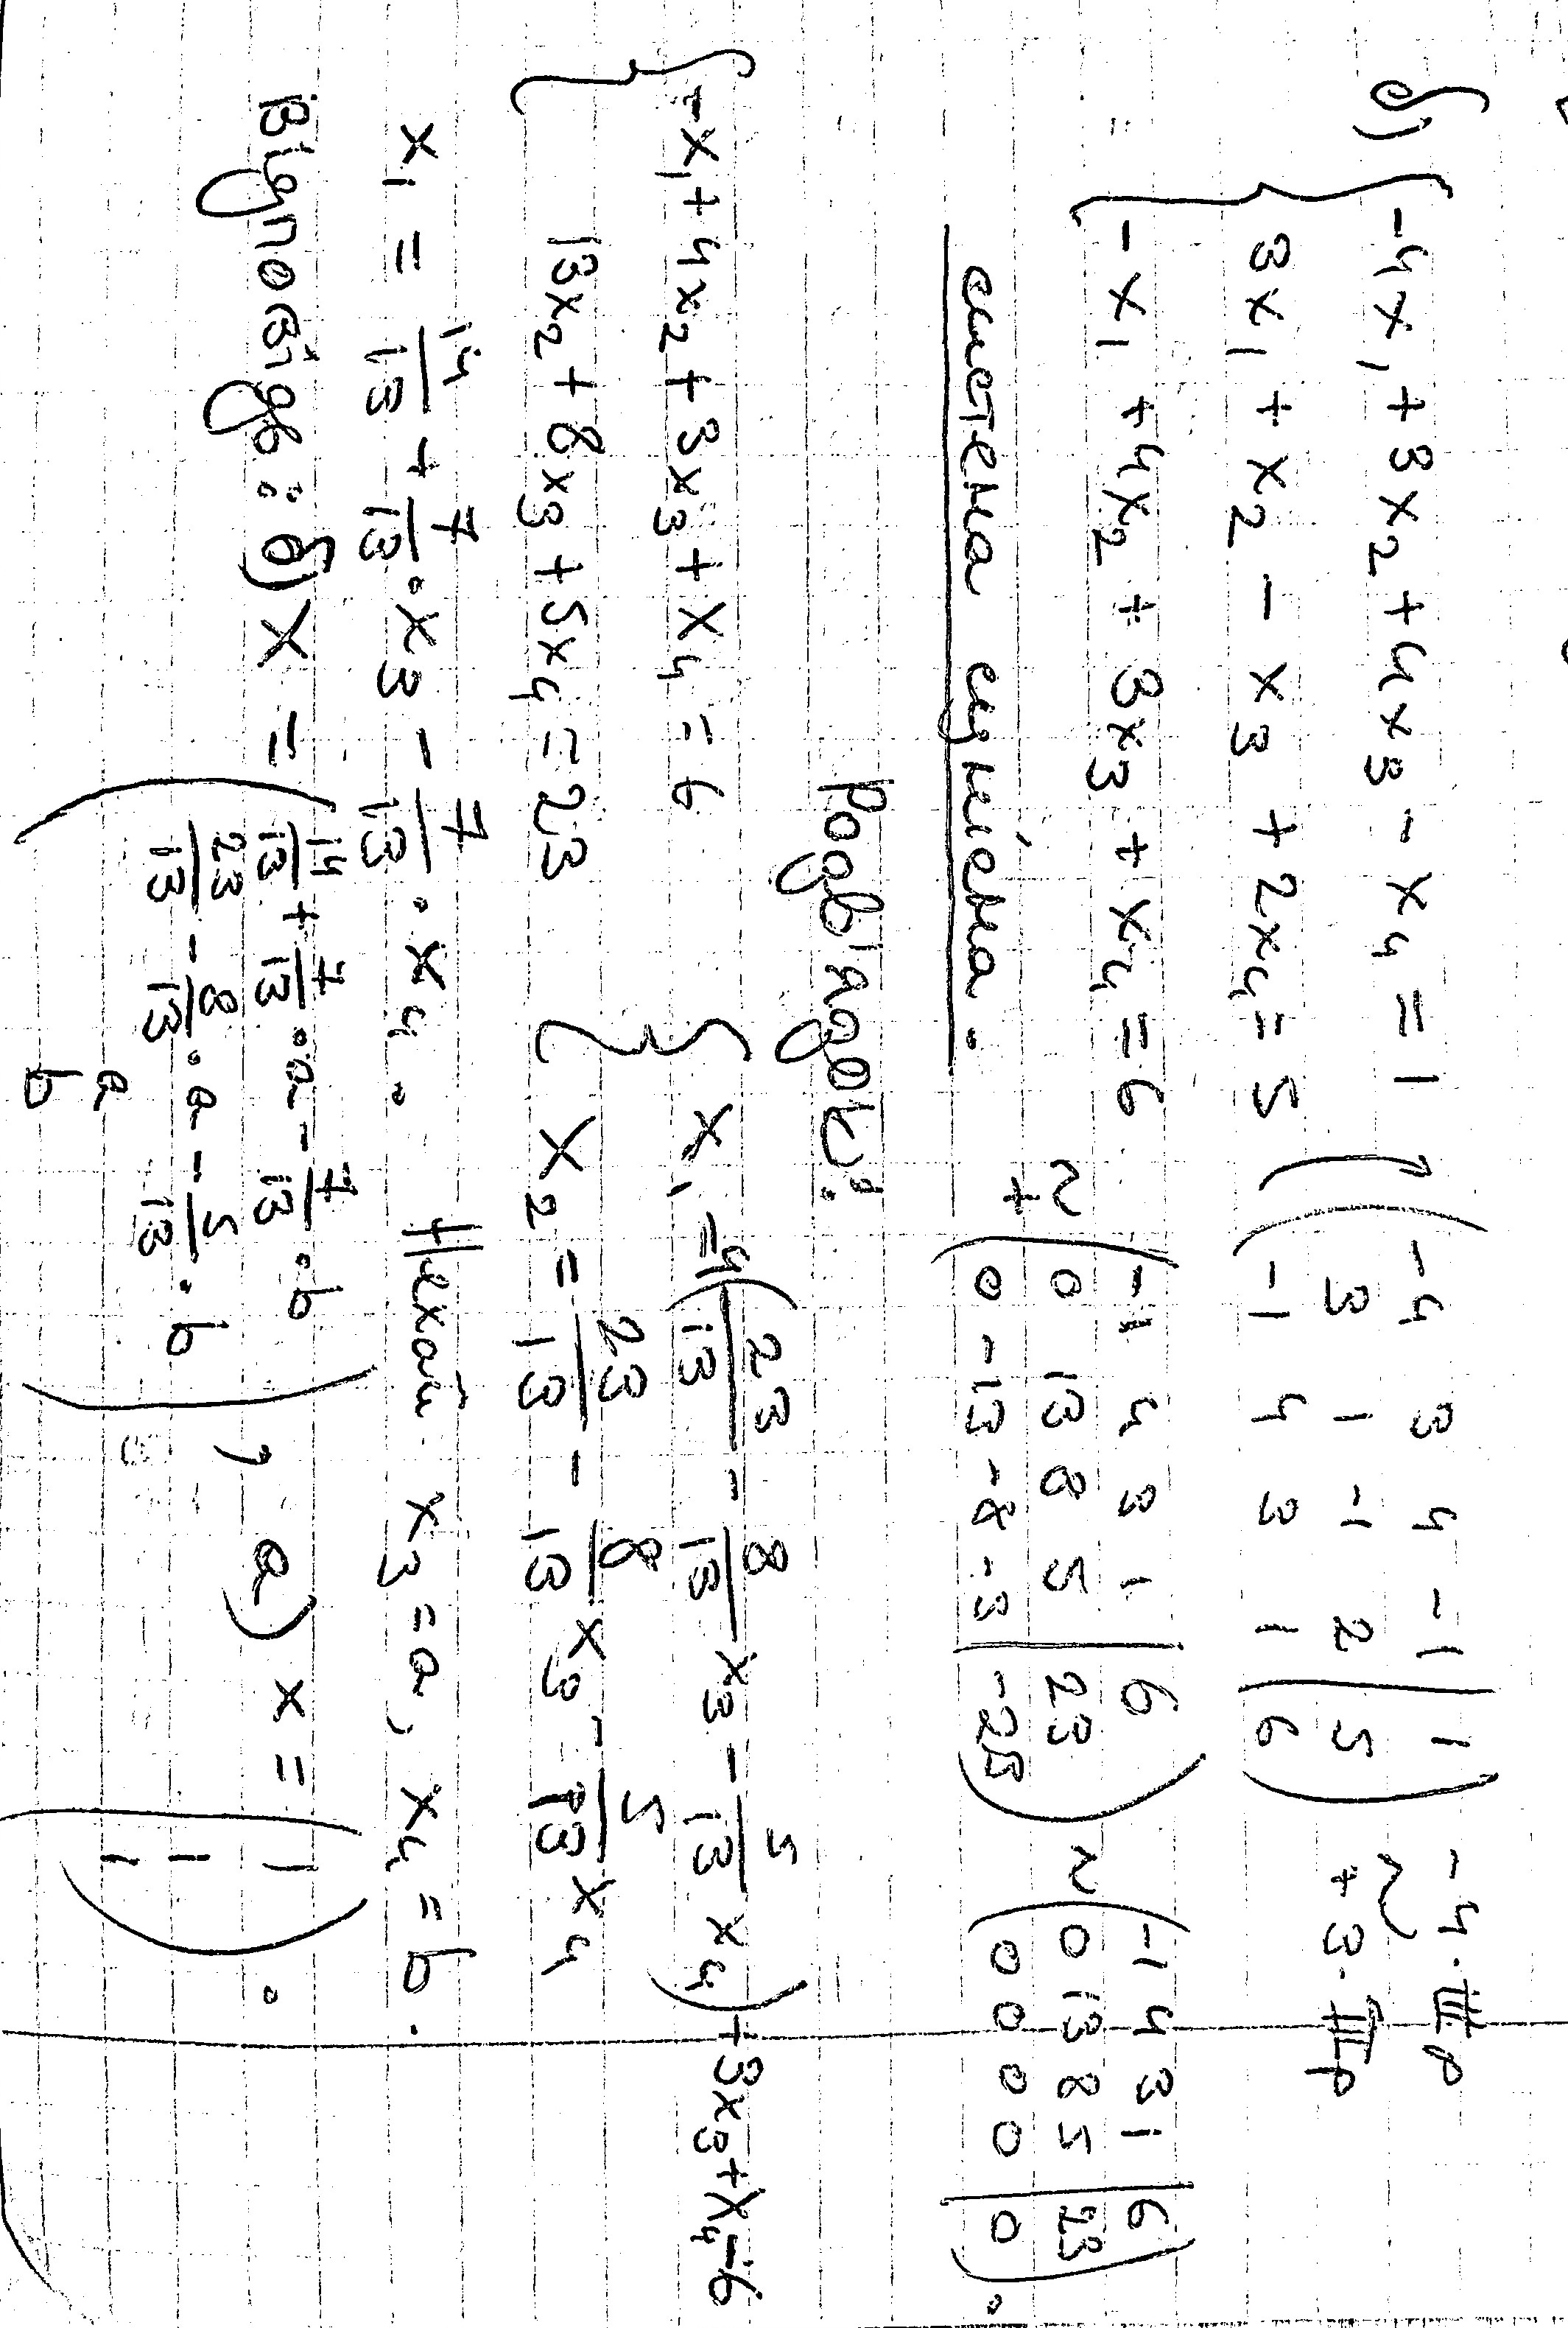
\includegraphics[width=12cm,angle=90]{ons/8.jpg}\\
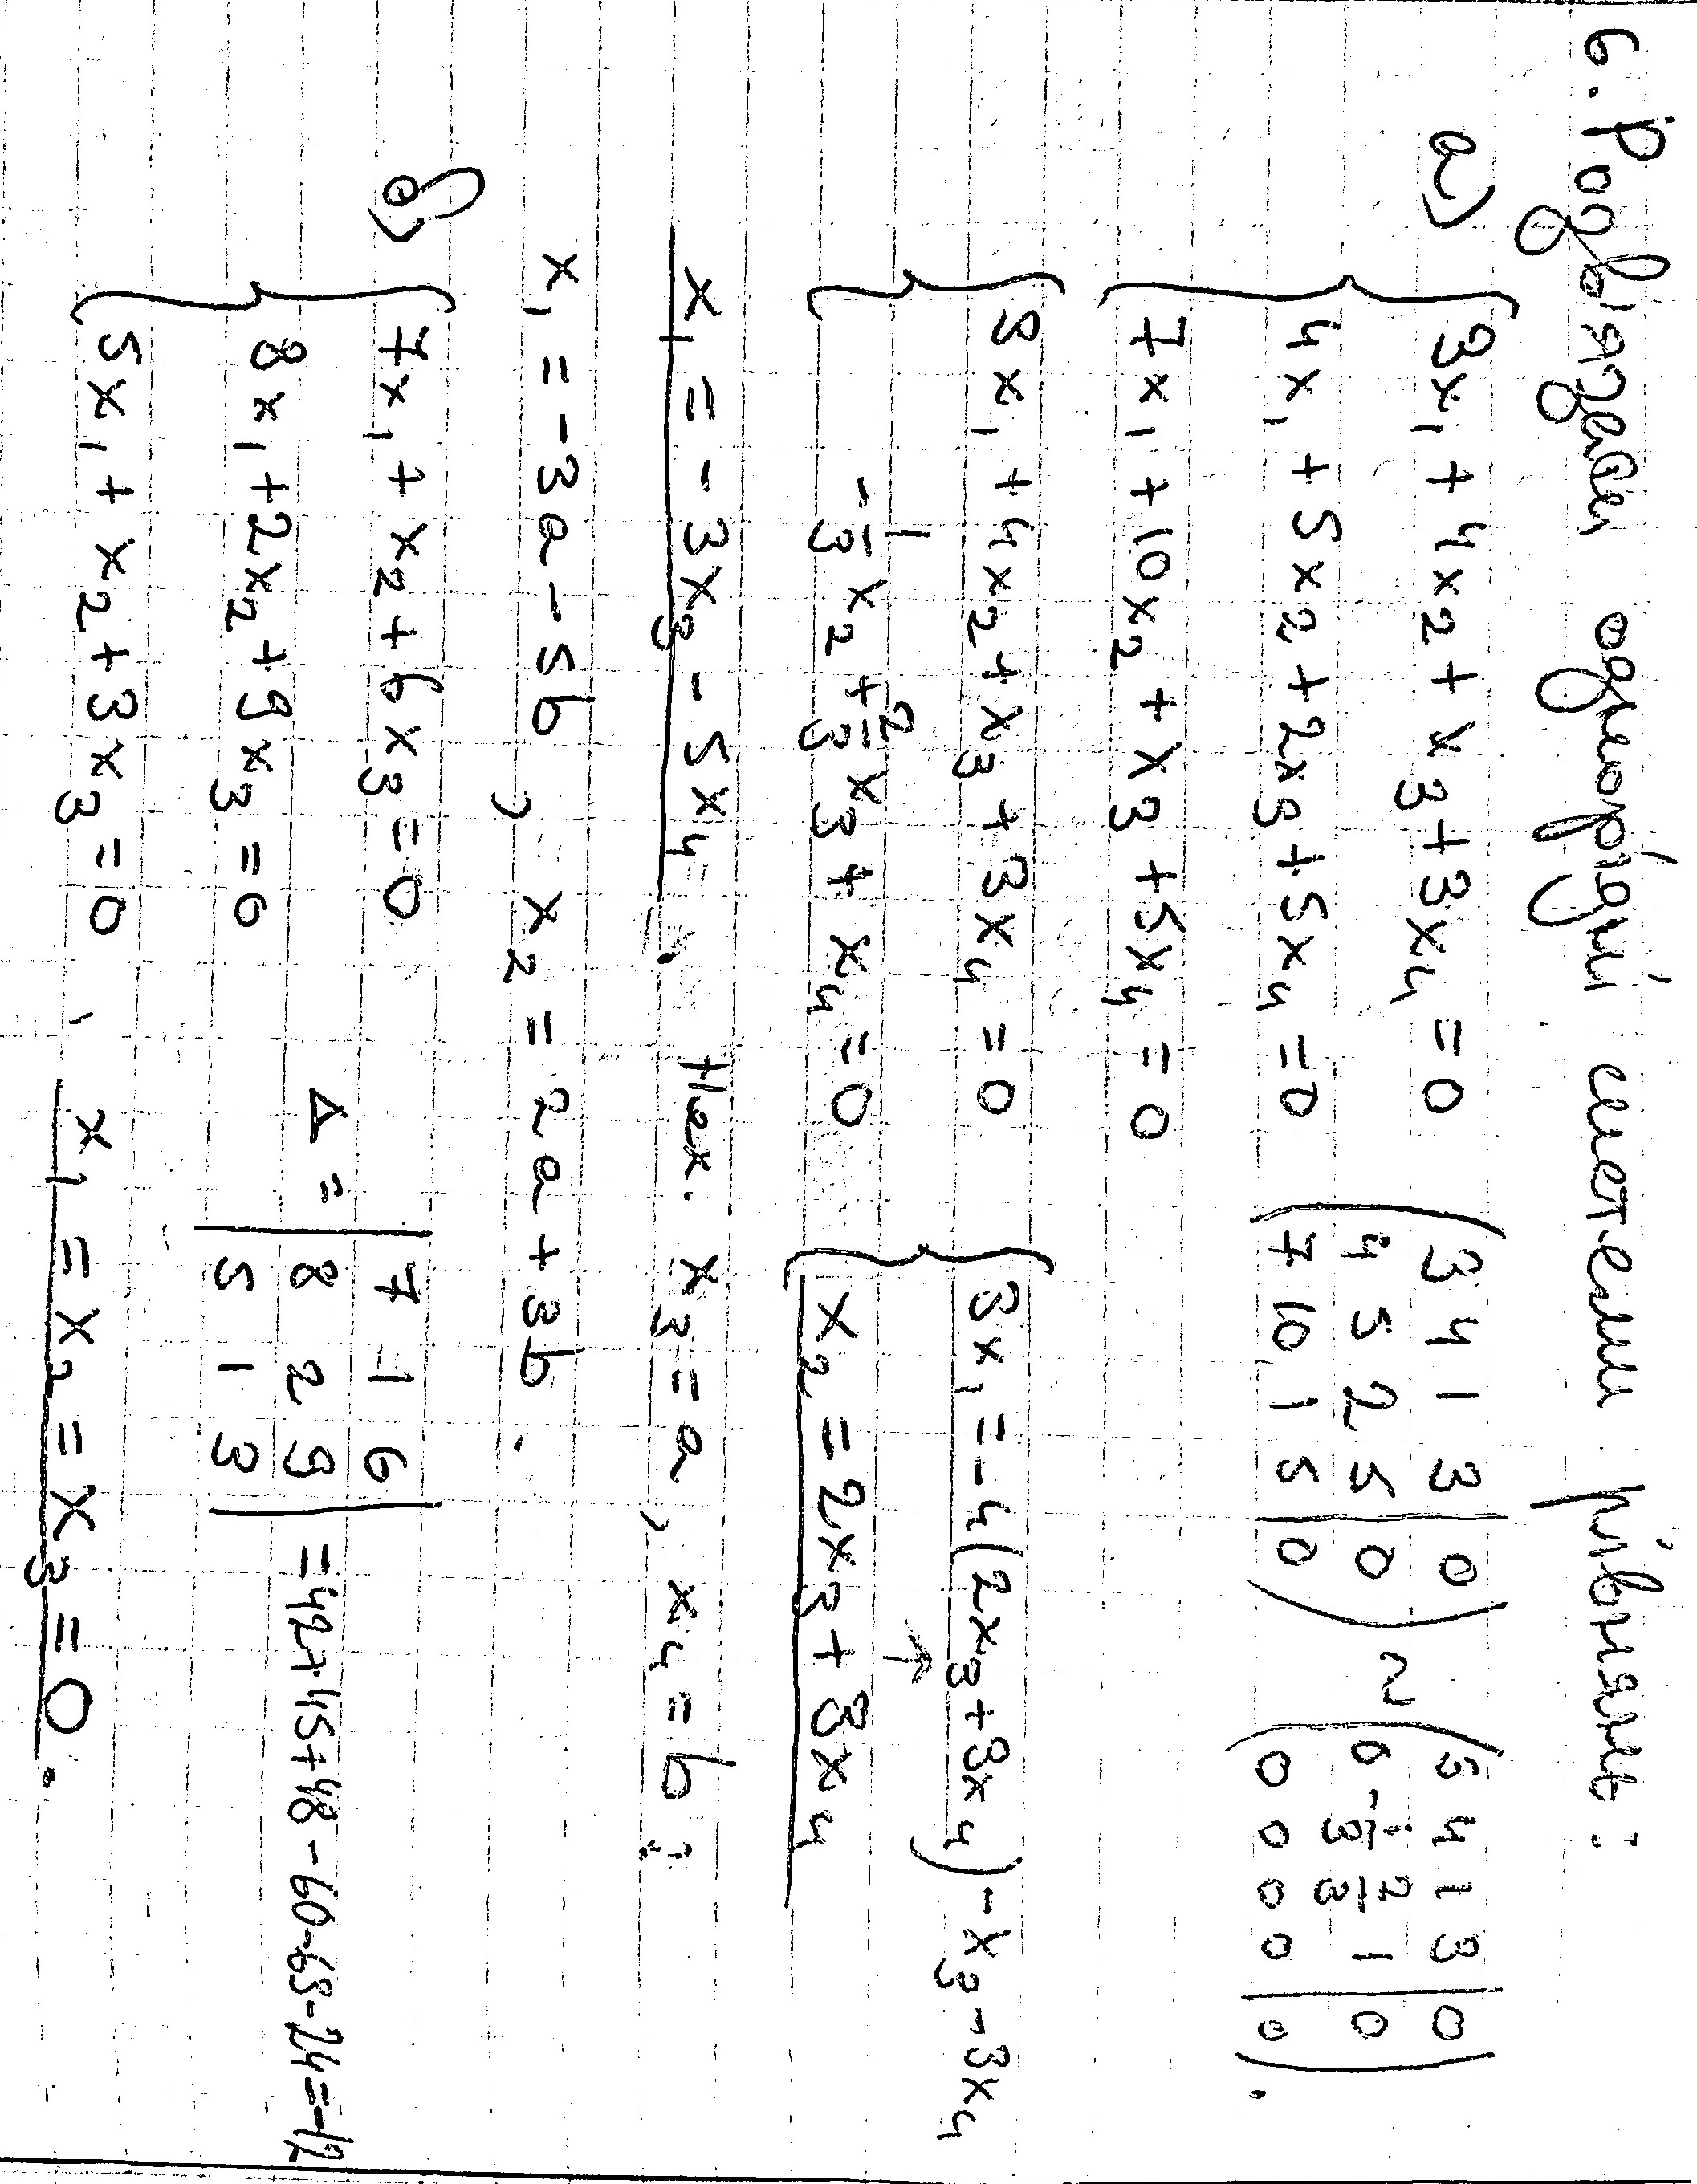
\includegraphics[width=13cm,angle=90]{ons/9.jpg}\\
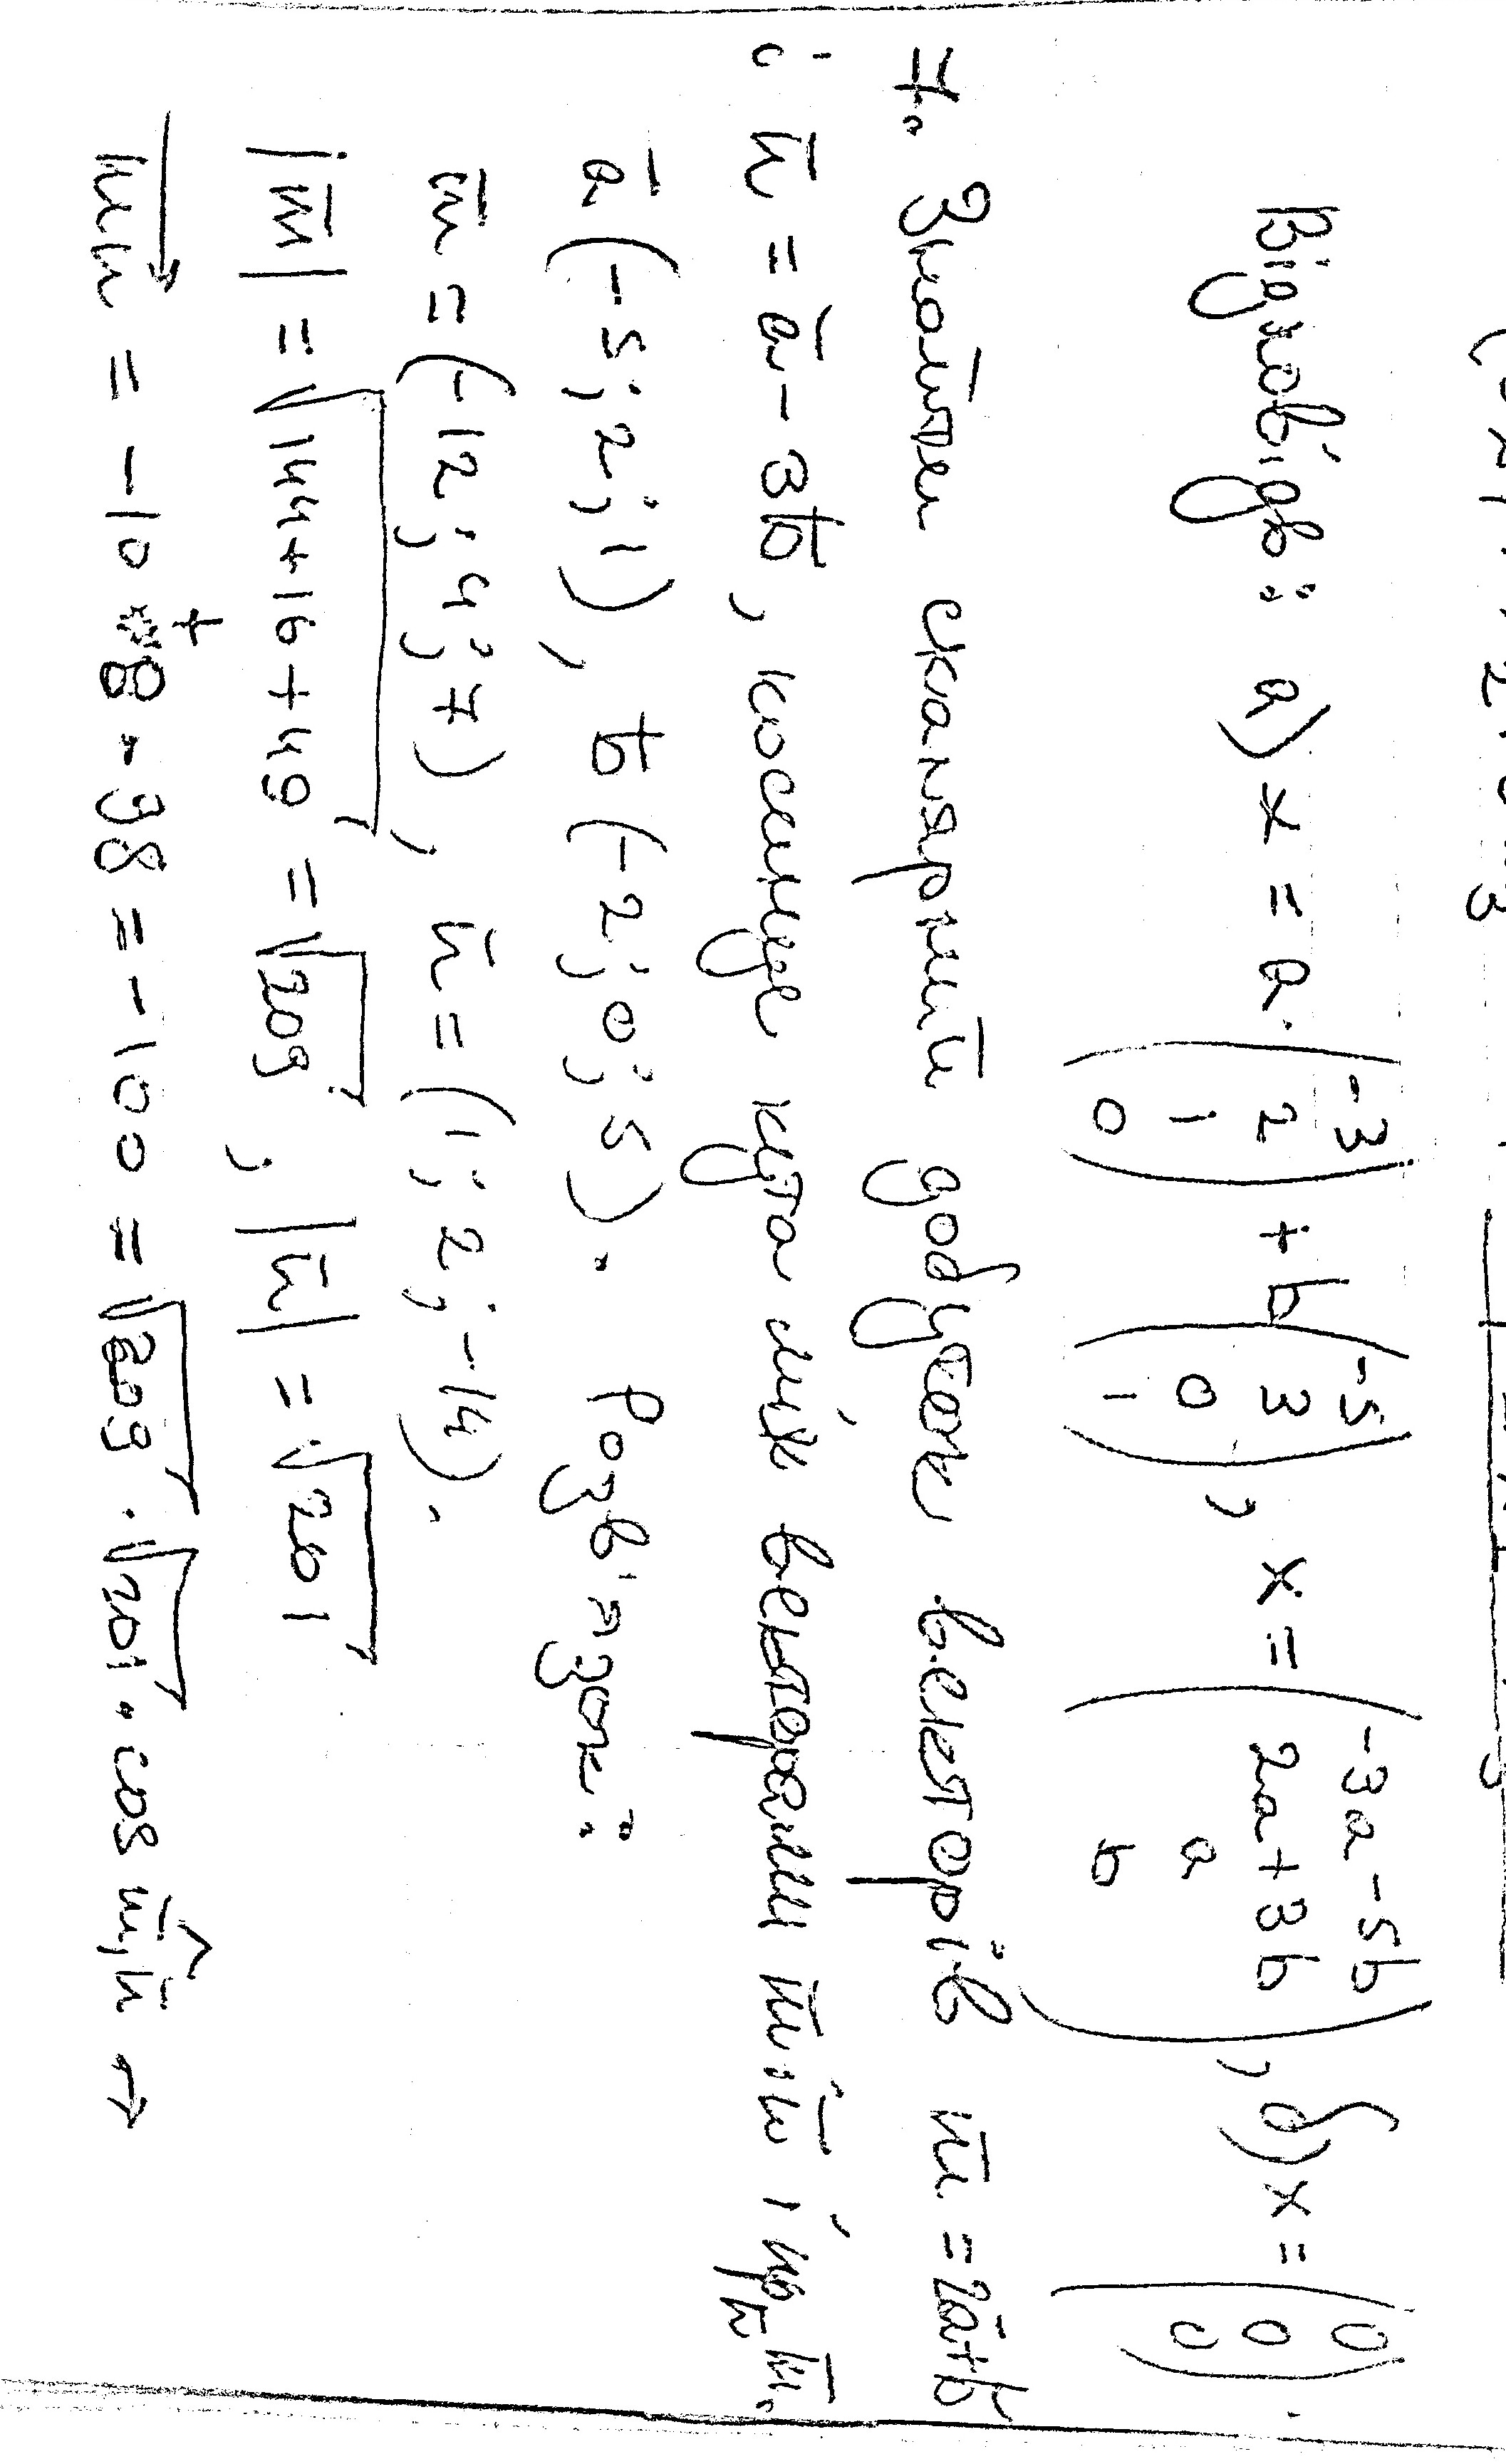
\includegraphics[width=11cm,angle=90]{ons/10.jpg}\\
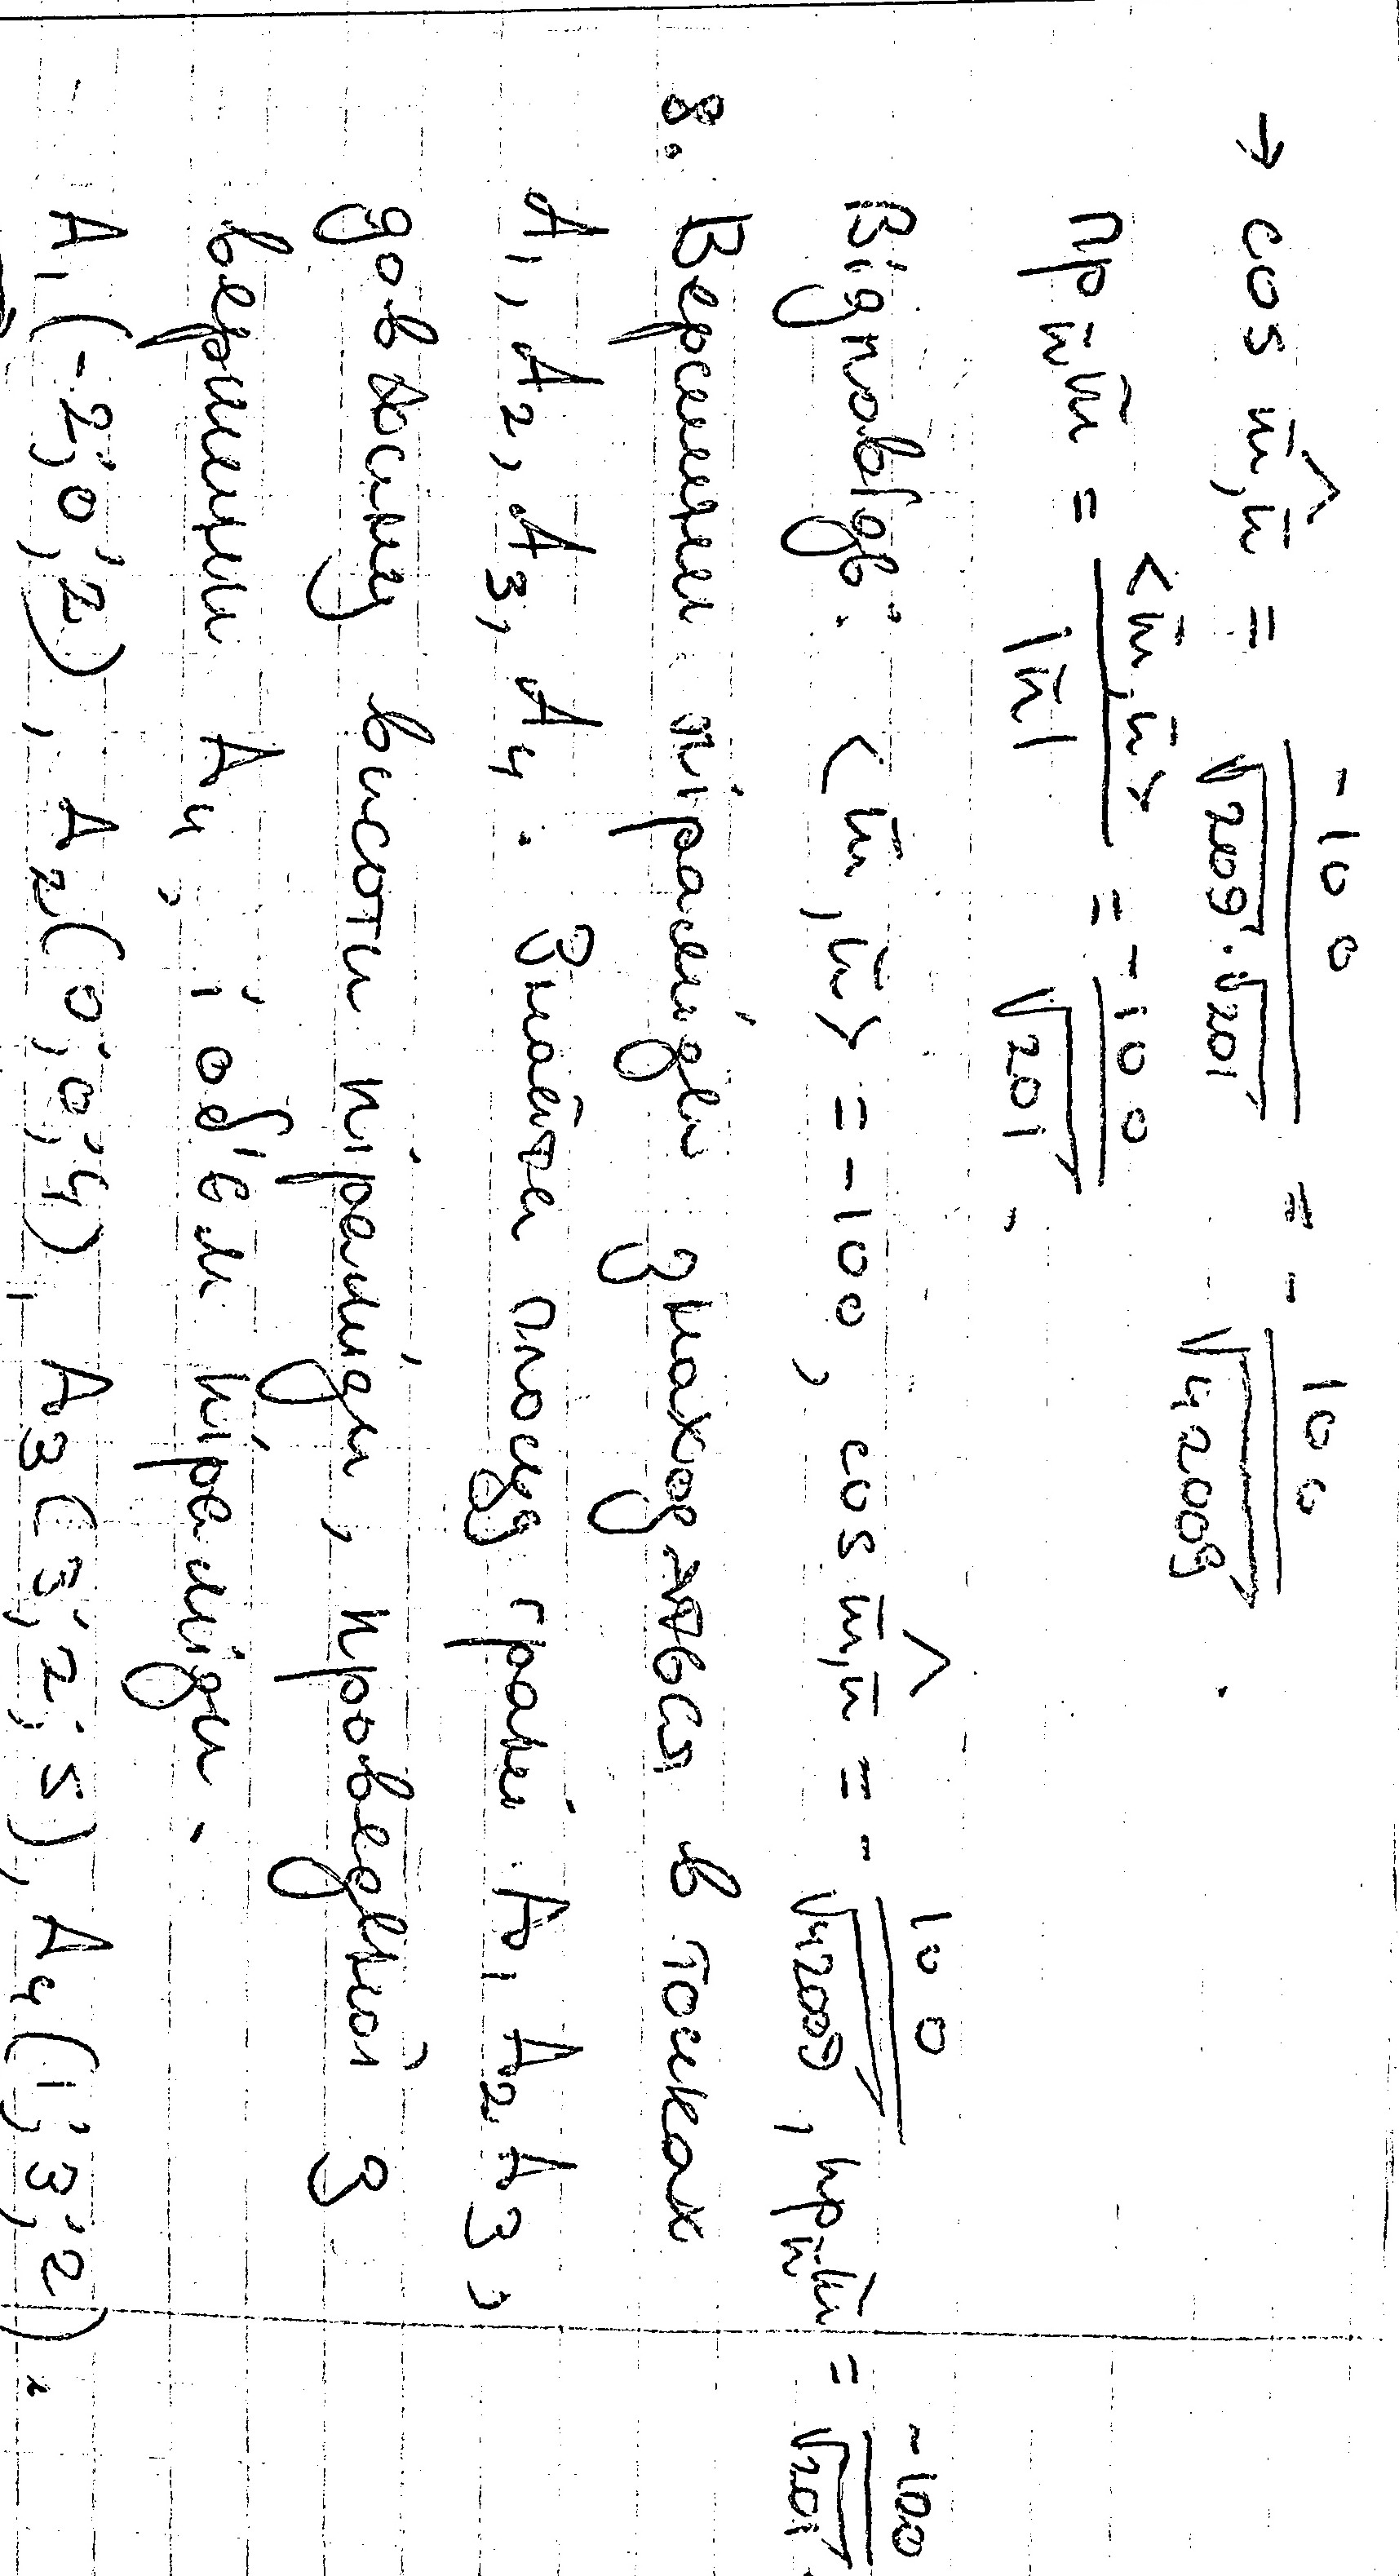
\includegraphics[width=10cm,angle=90]{ons/11.jpg}\\
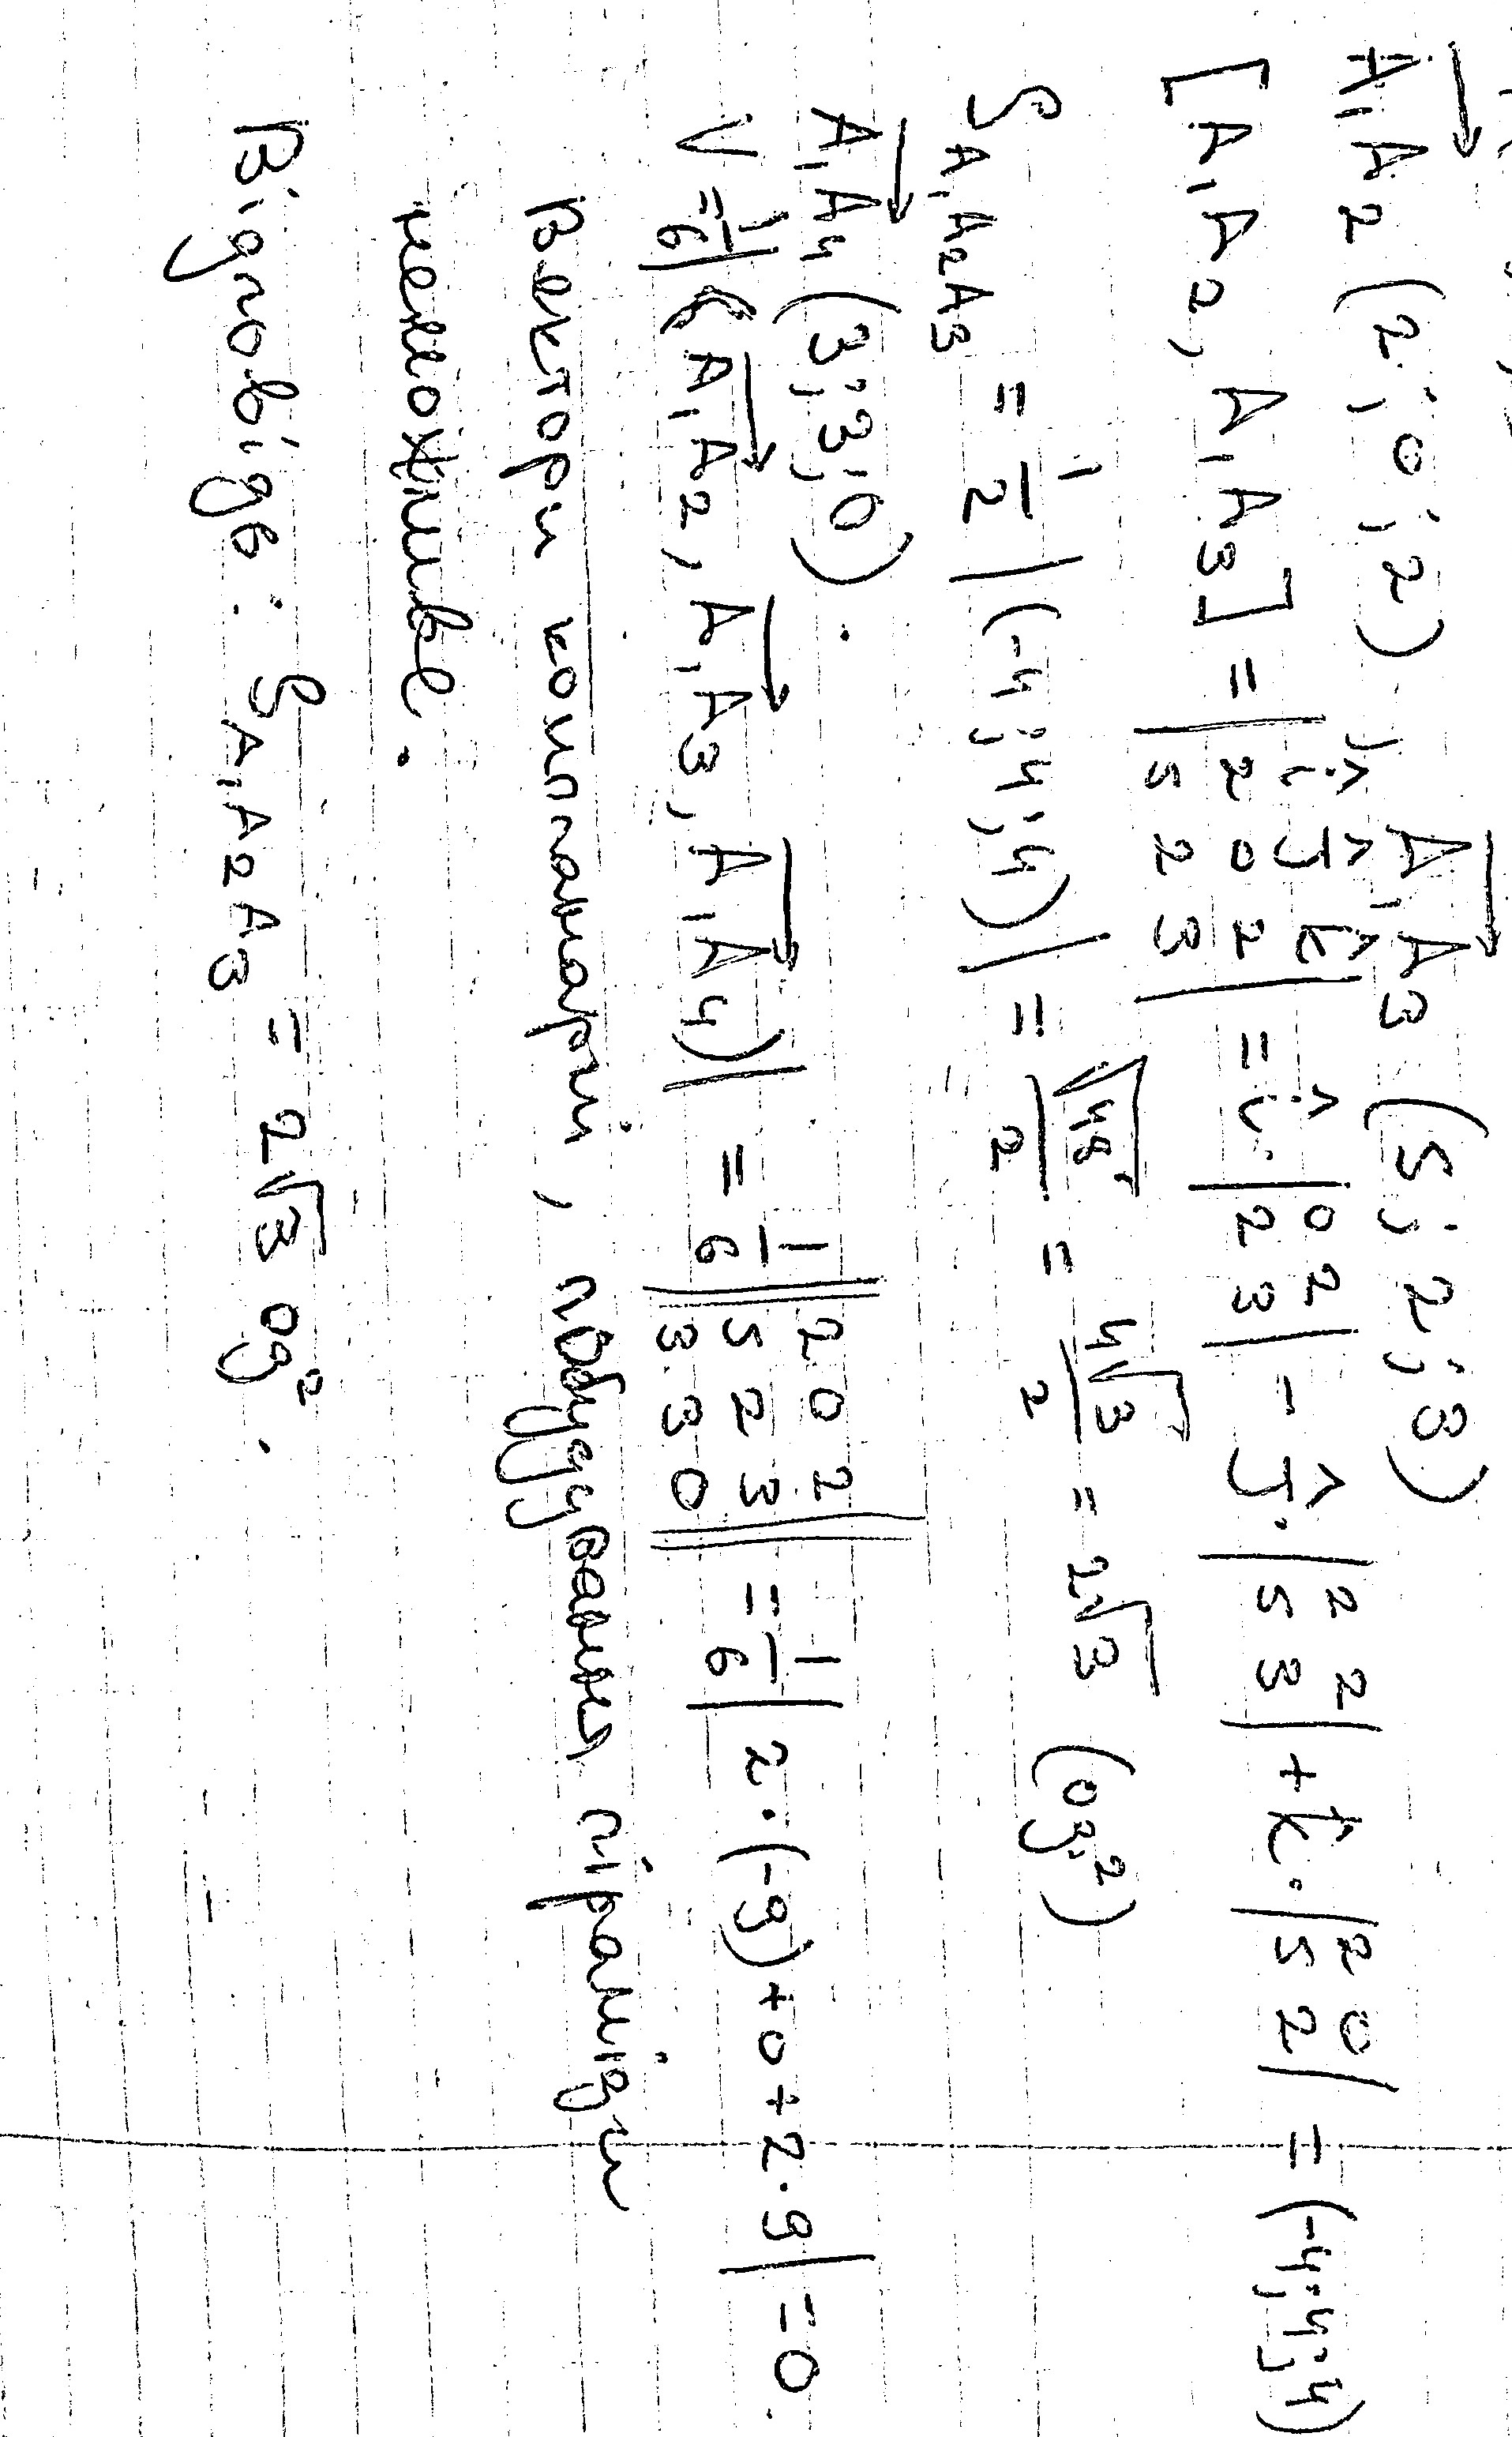
\includegraphics[width=11cm,angle=90]{ons/12.jpg}\\
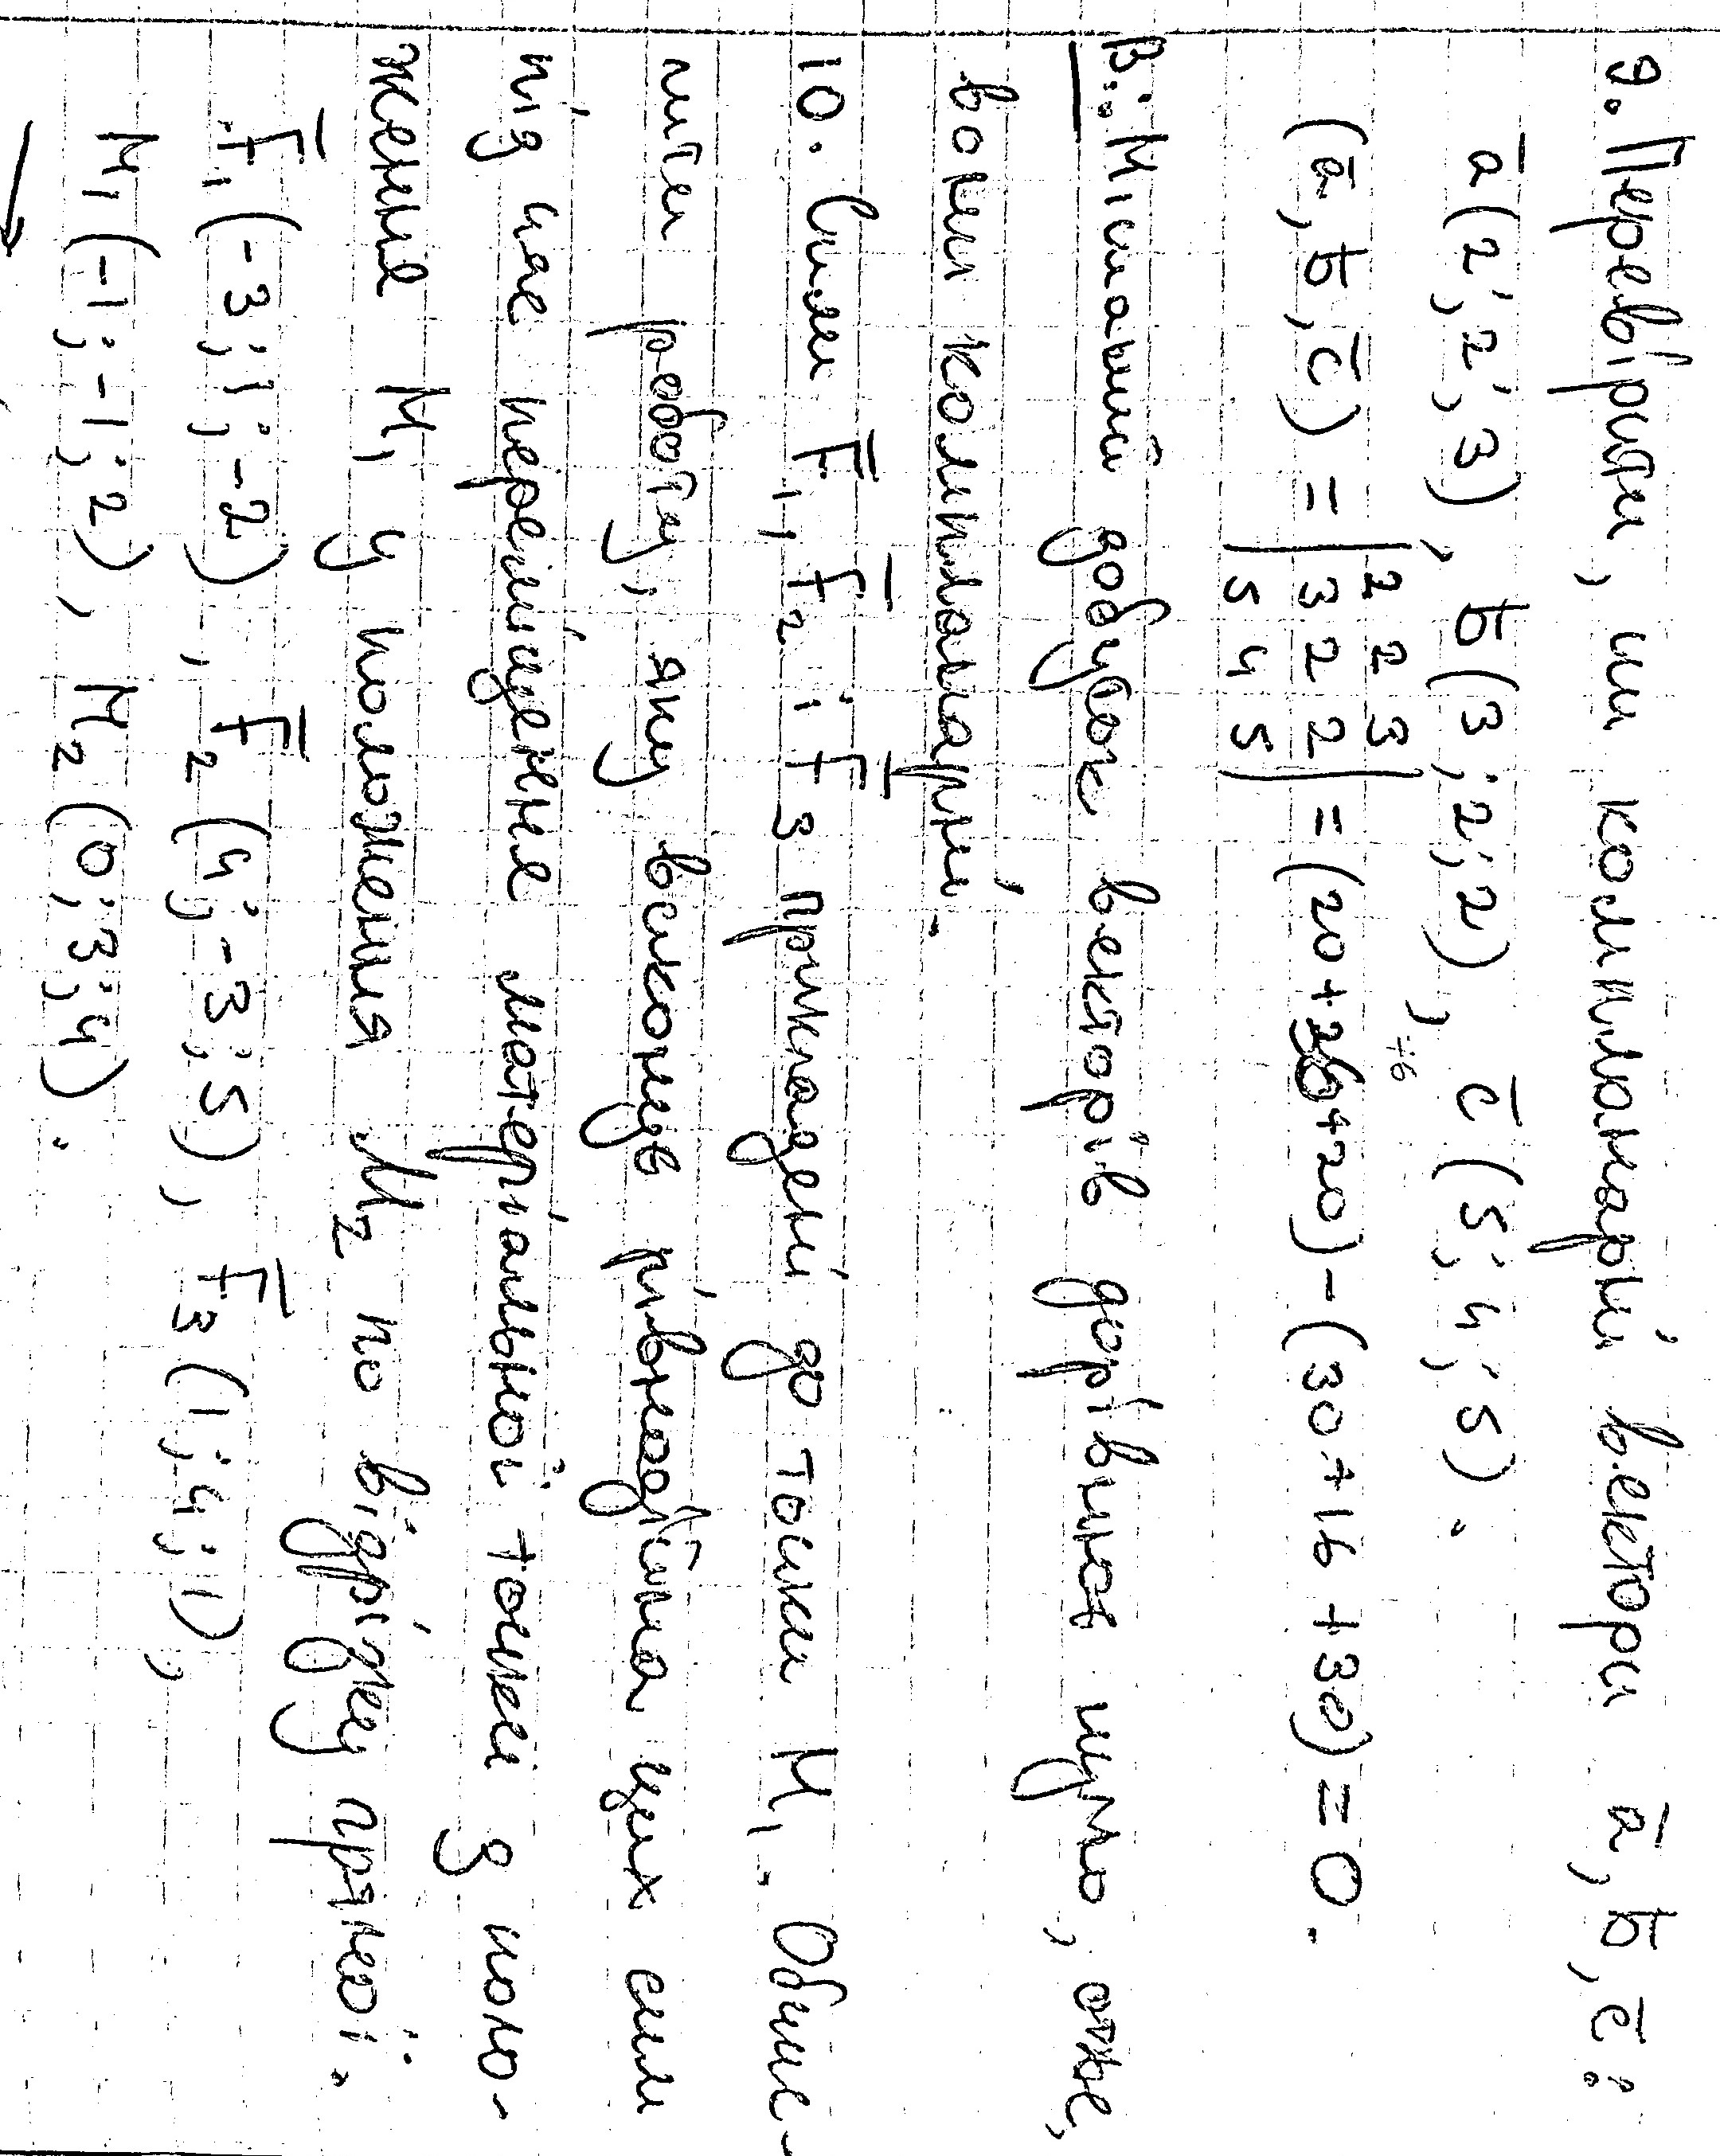
\includegraphics[width=13cm,angle=90]{ons/13.jpg}\\
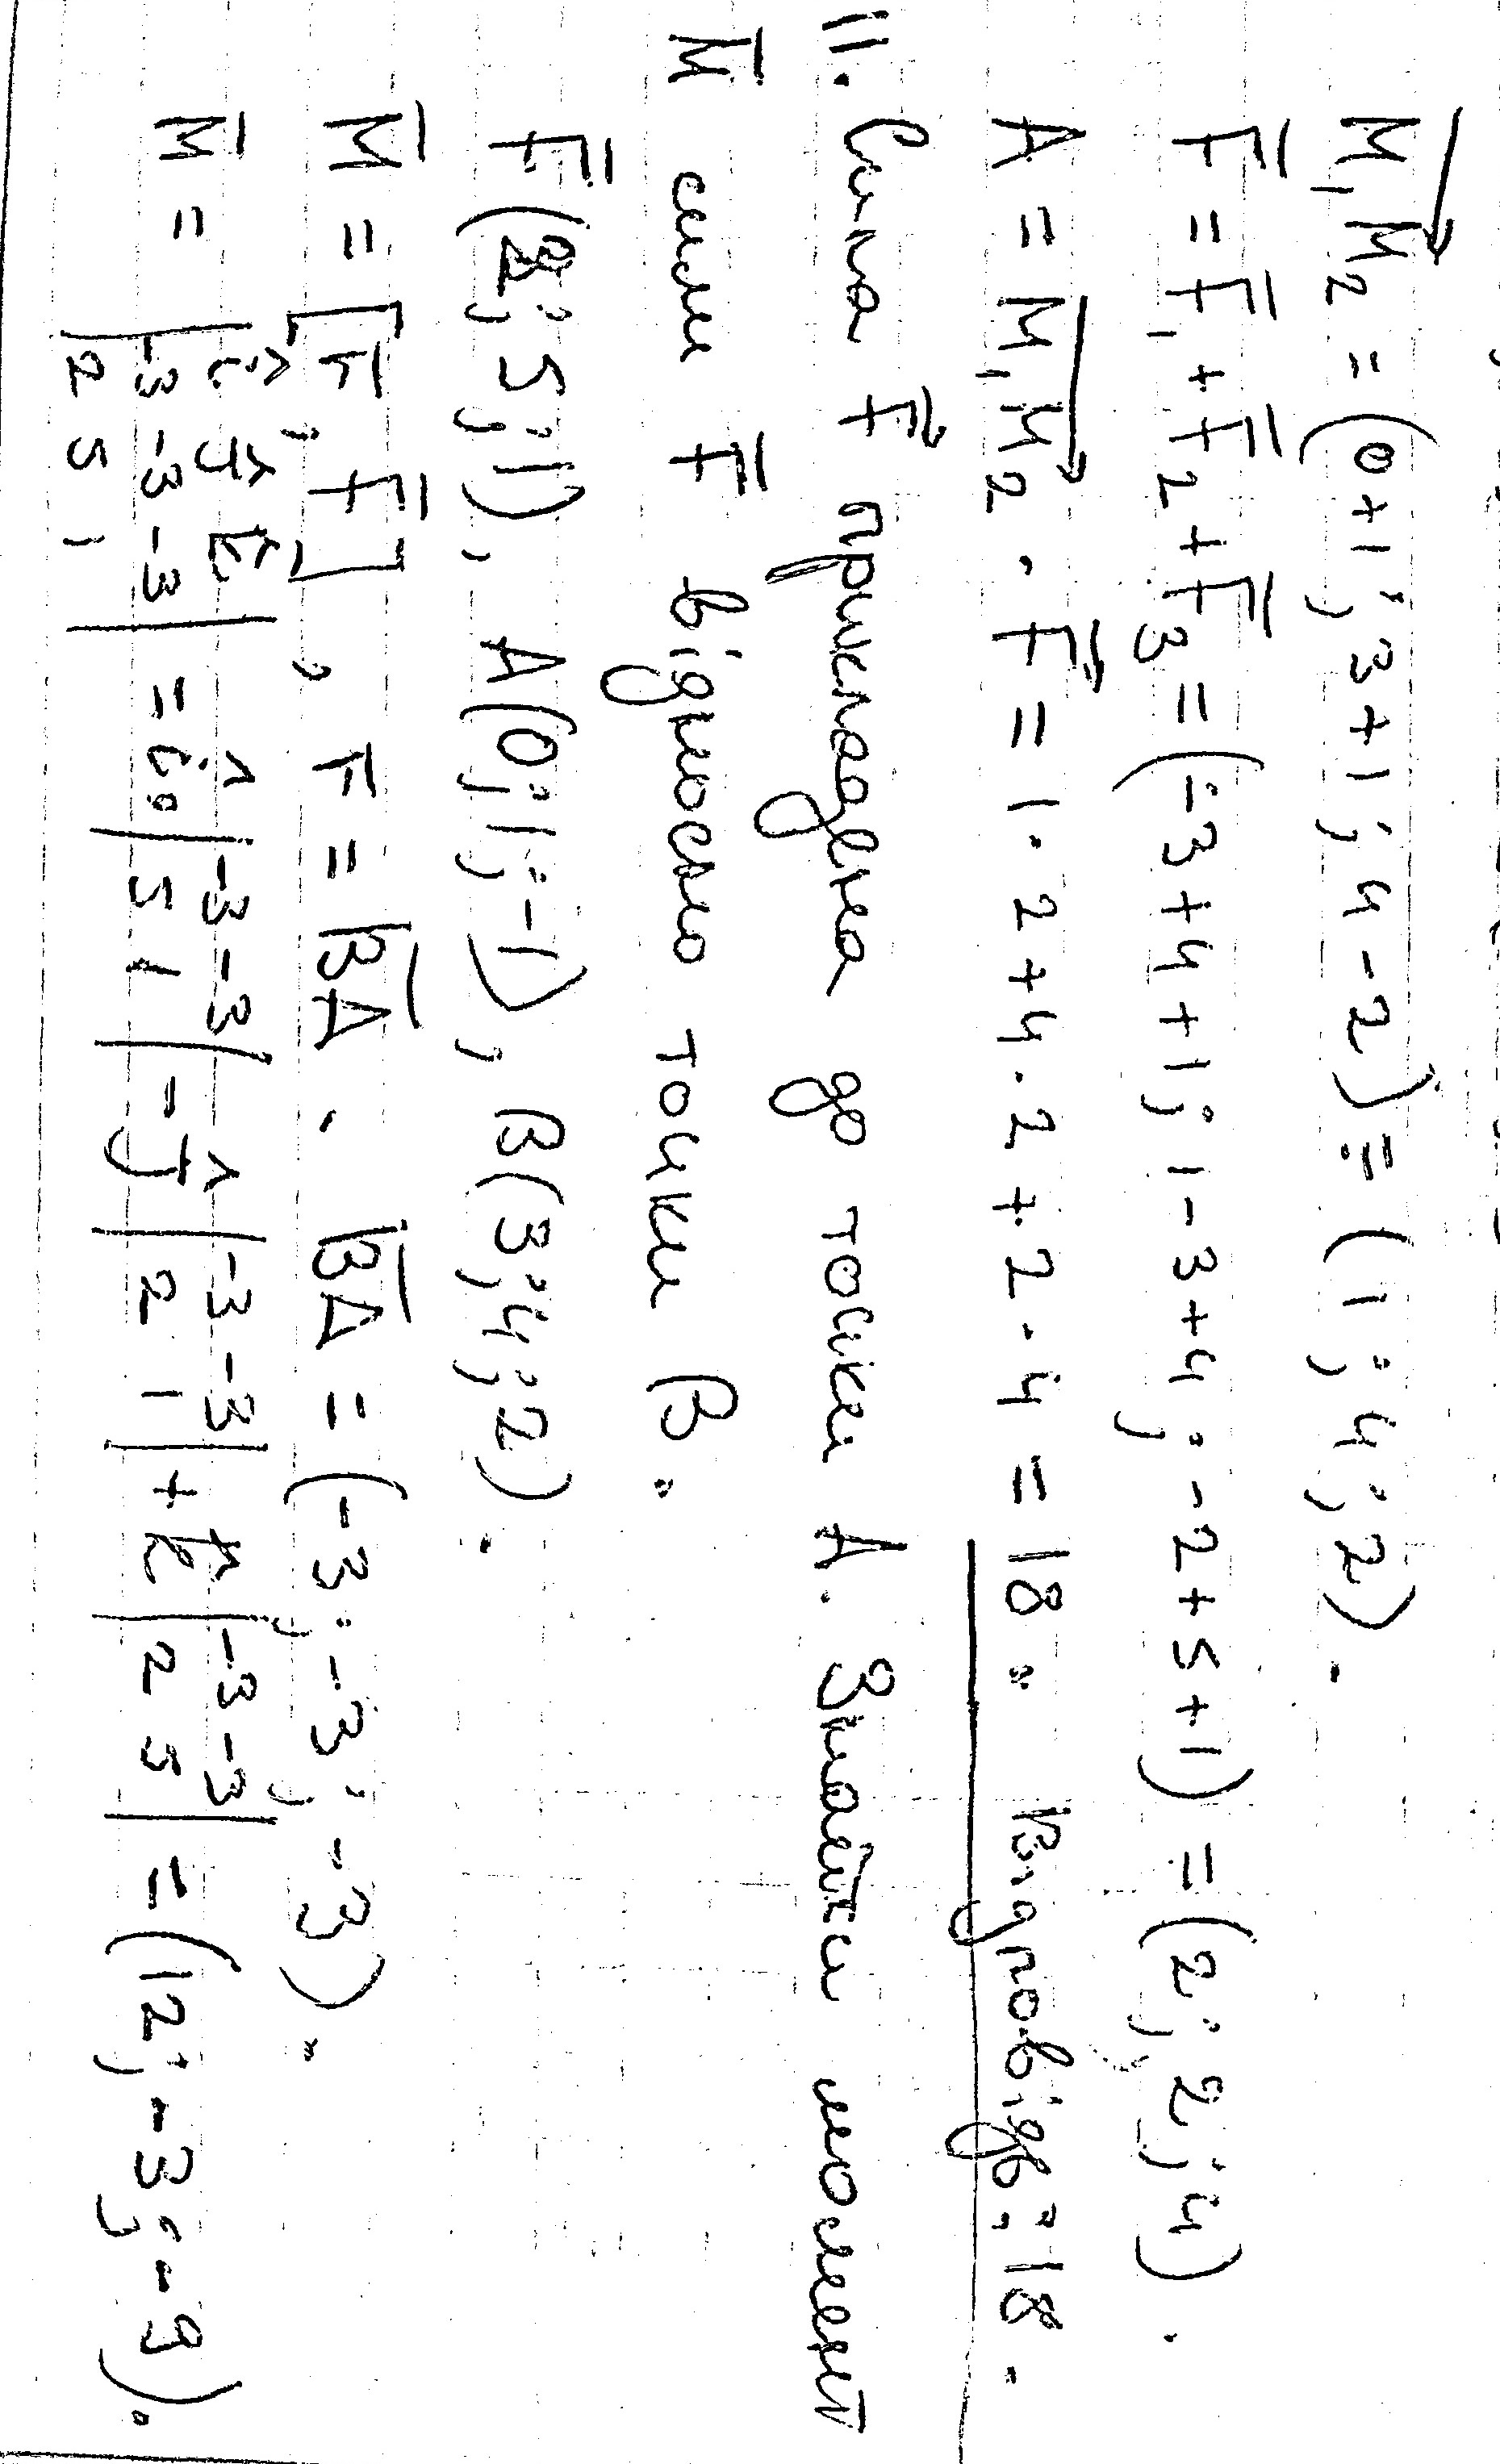
\includegraphics[width=11cm,angle=90]{ons/14.jpg}\\
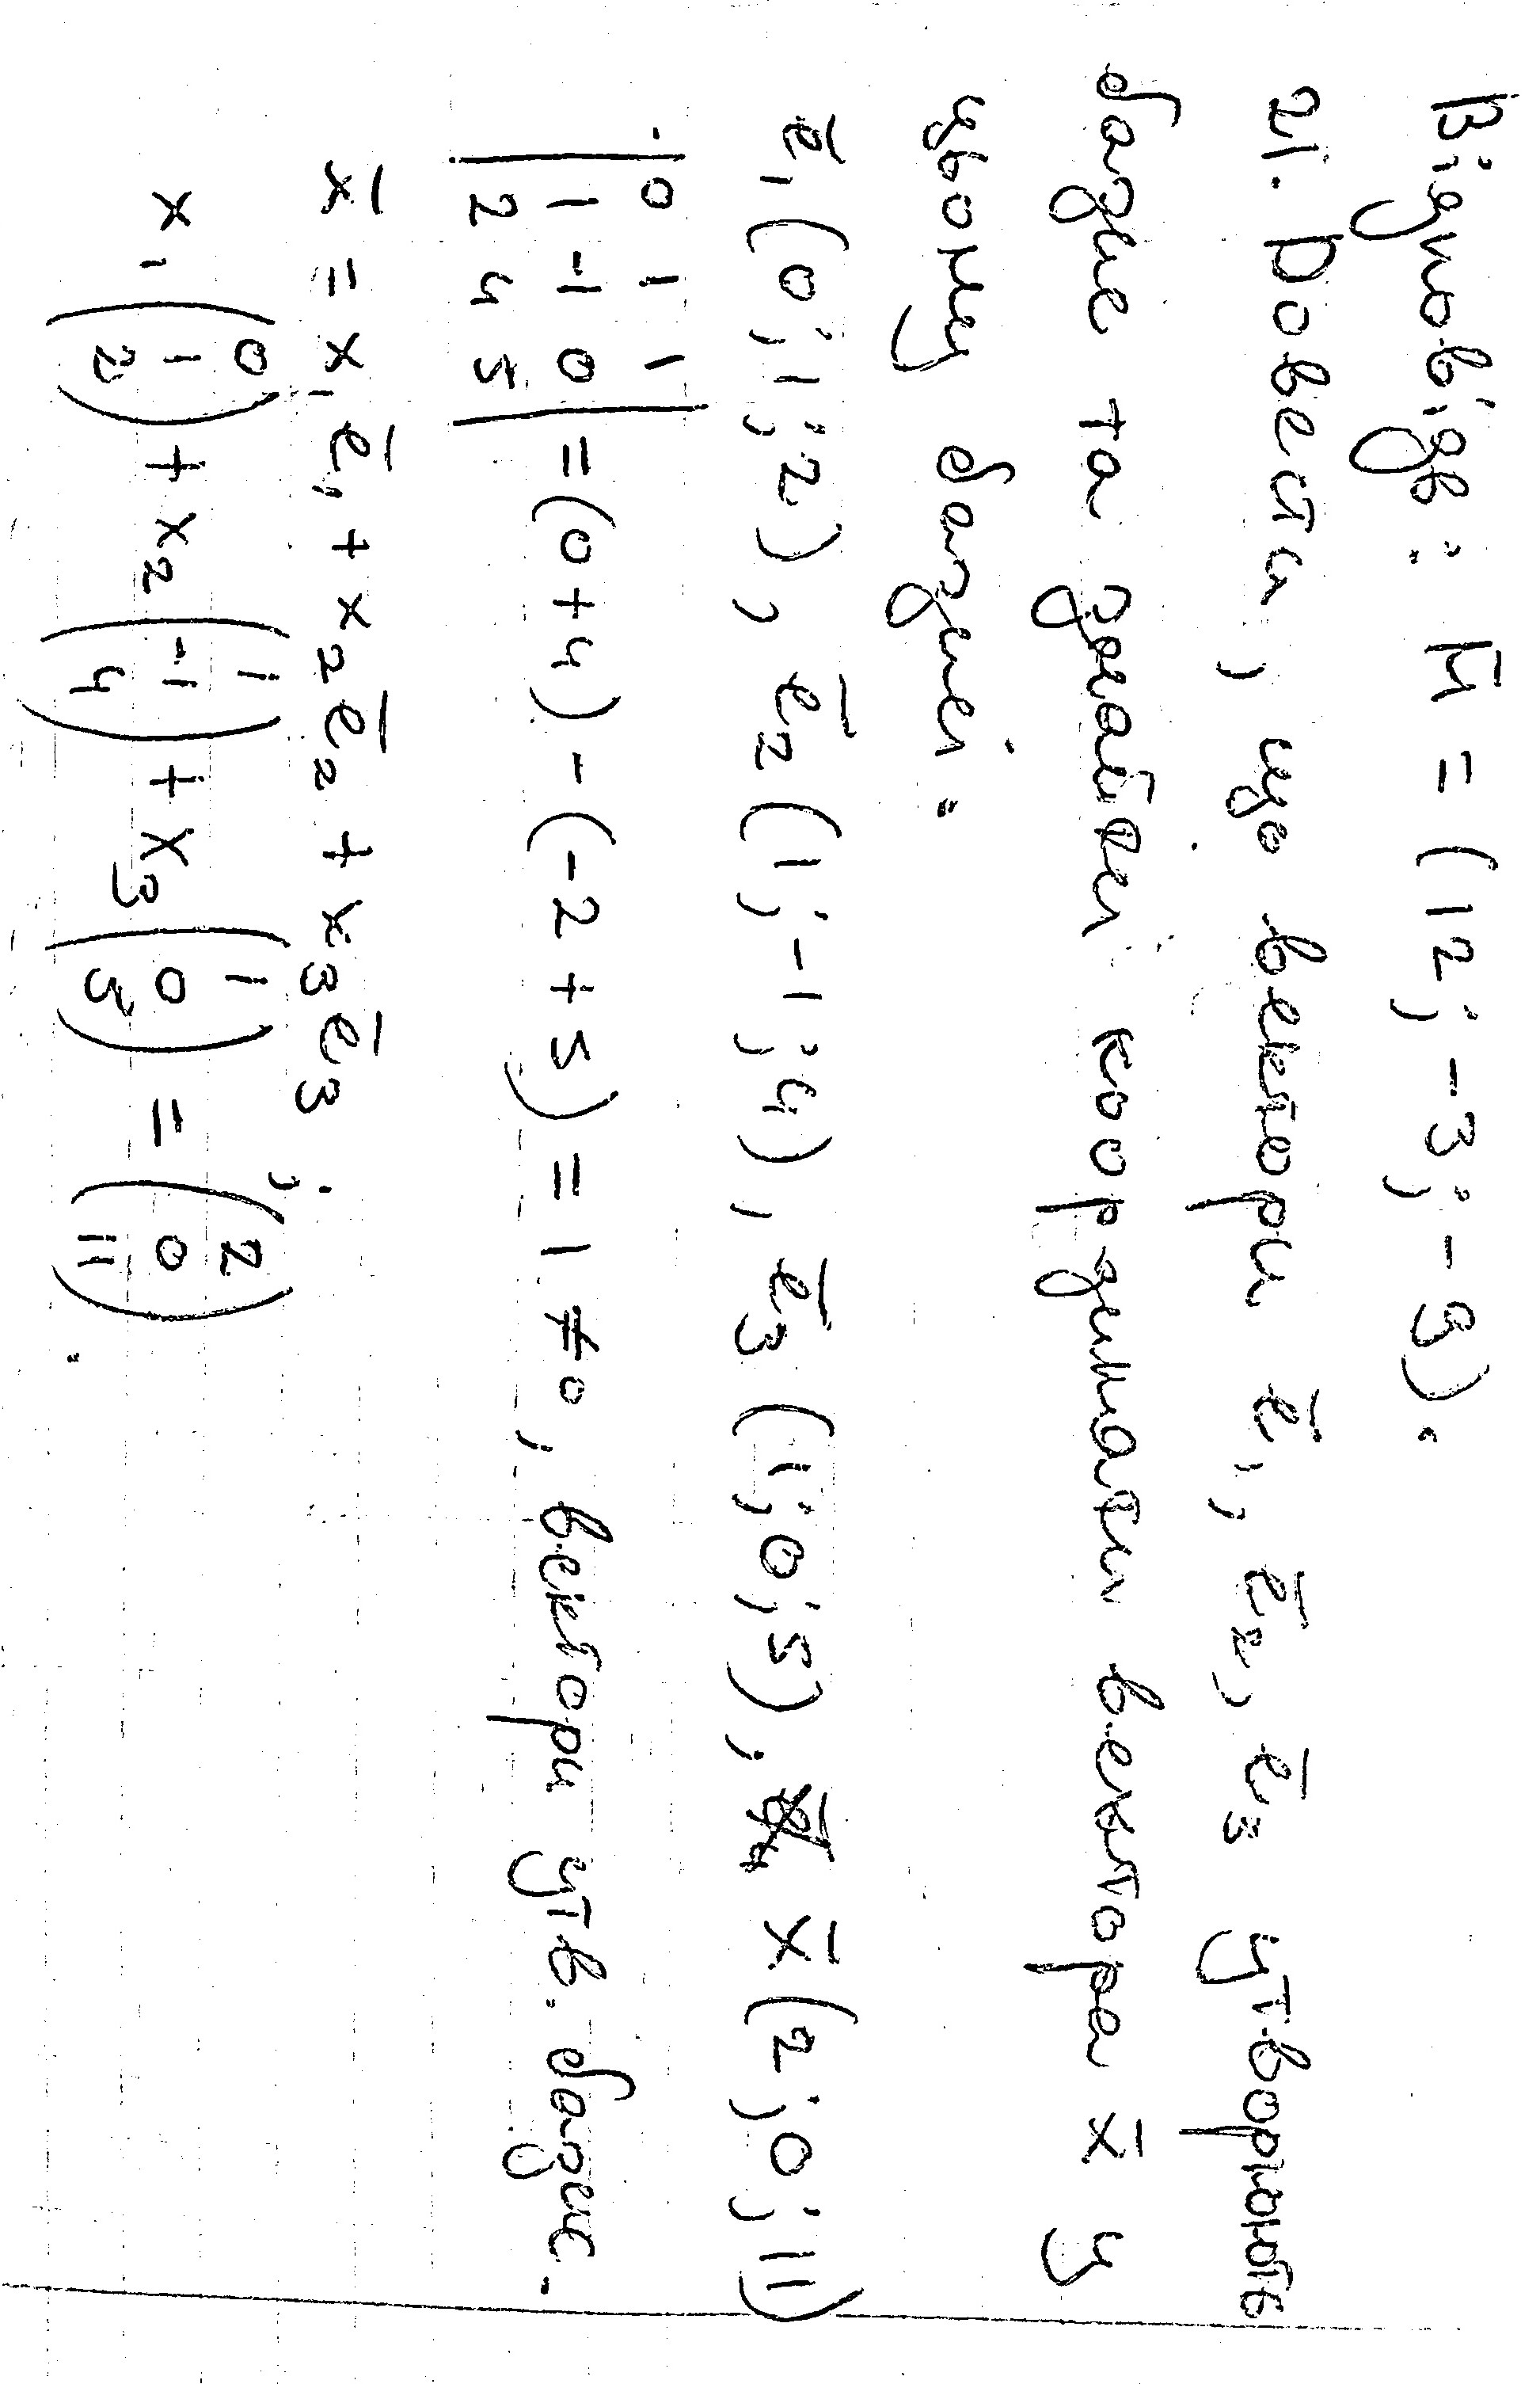
\includegraphics[width=12cm,angle=90]{ons/15.jpg}\\
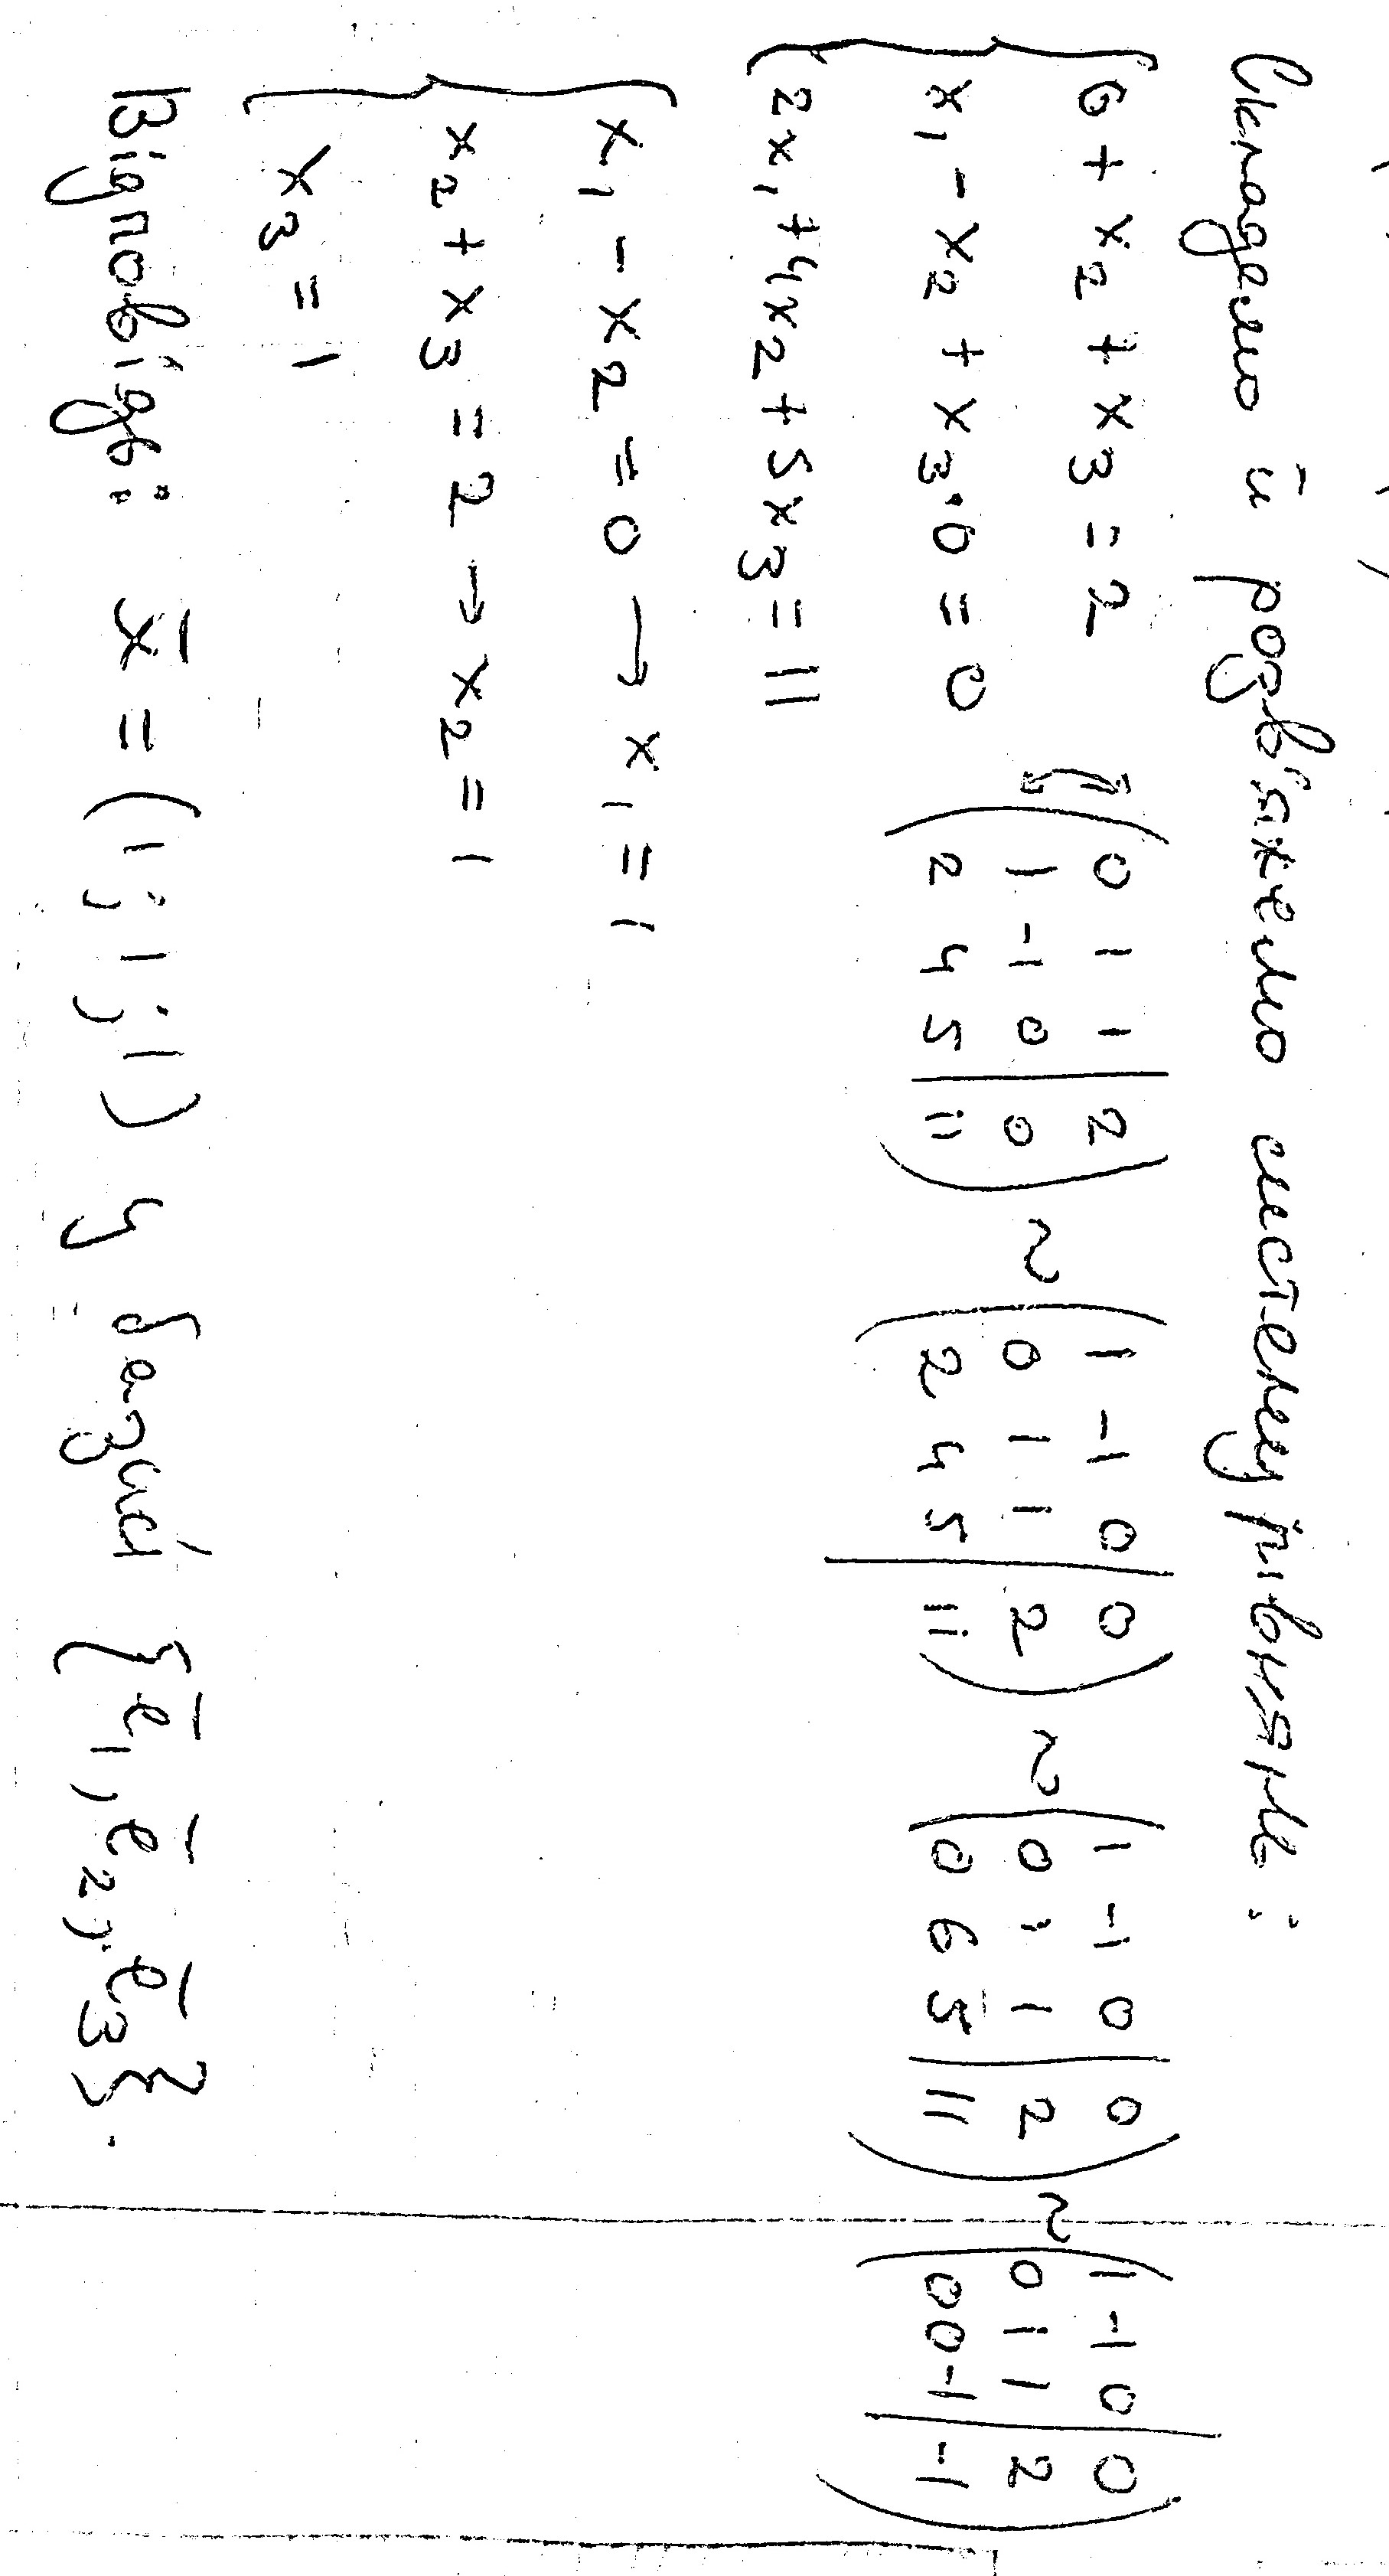
\includegraphics[width=10cm,angle=90]{ons/16.jpg}\\
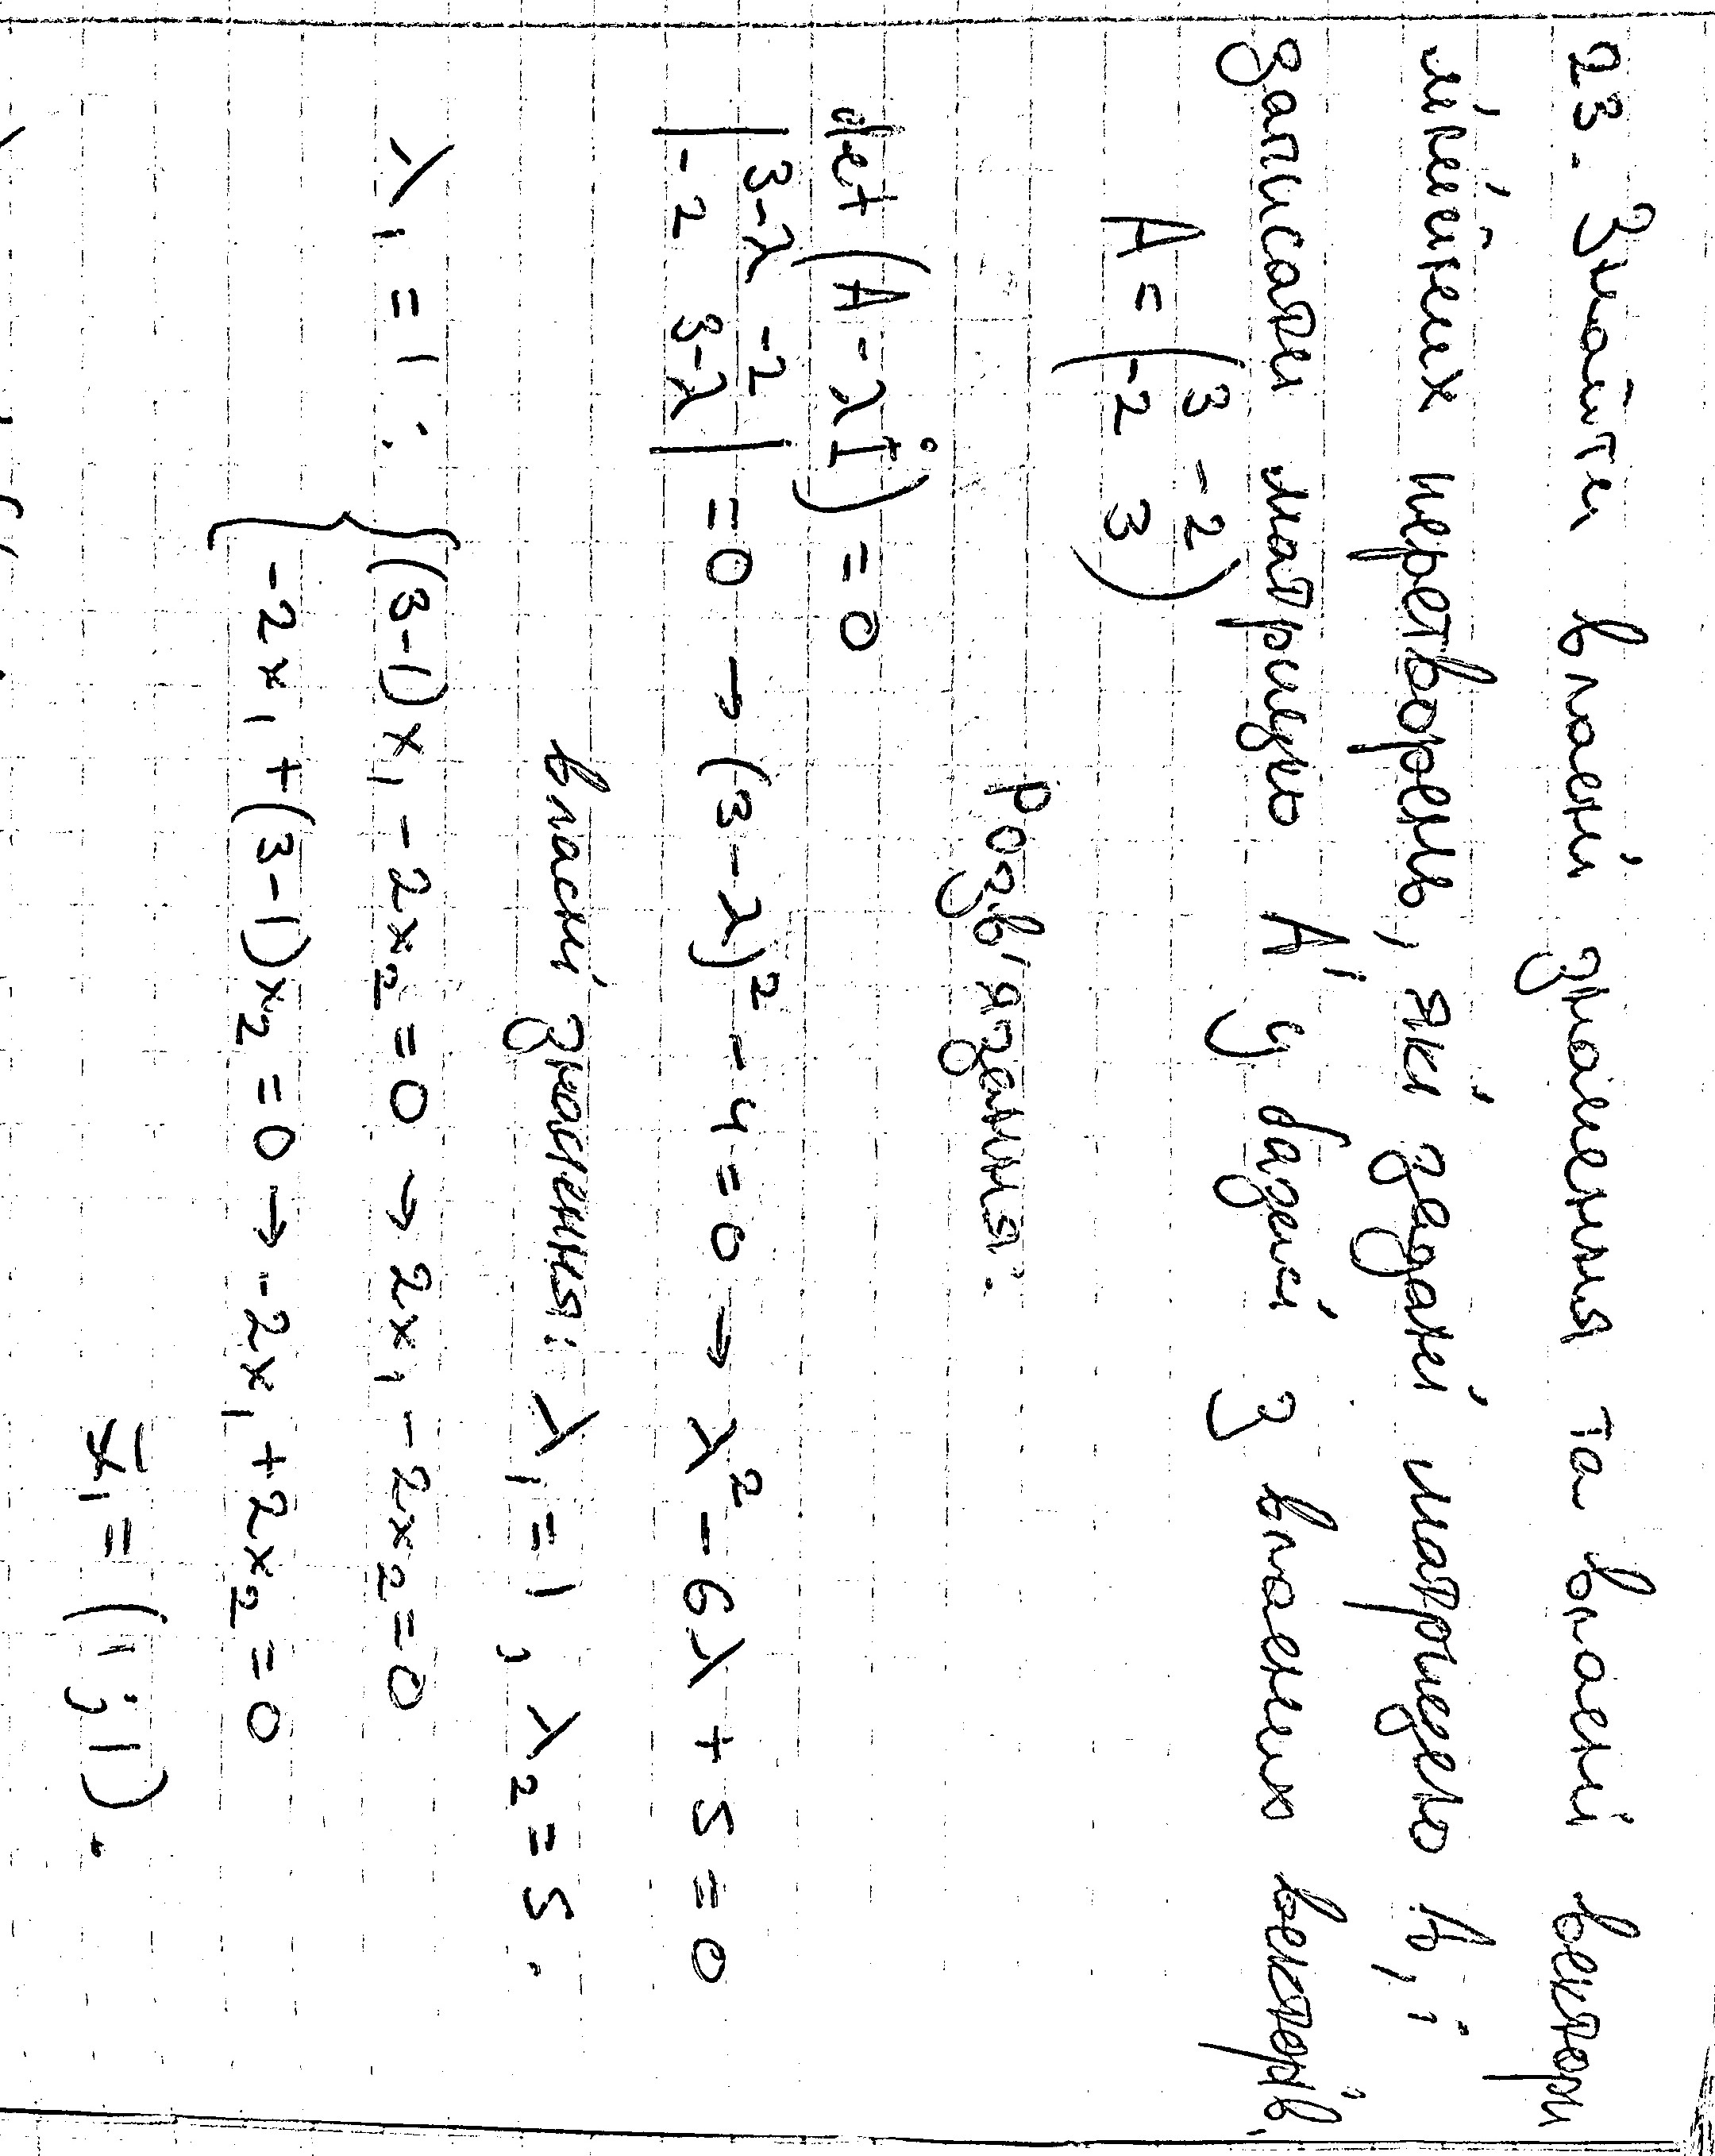
\includegraphics[width=14cm,angle=90]{ons/17.jpg}\\
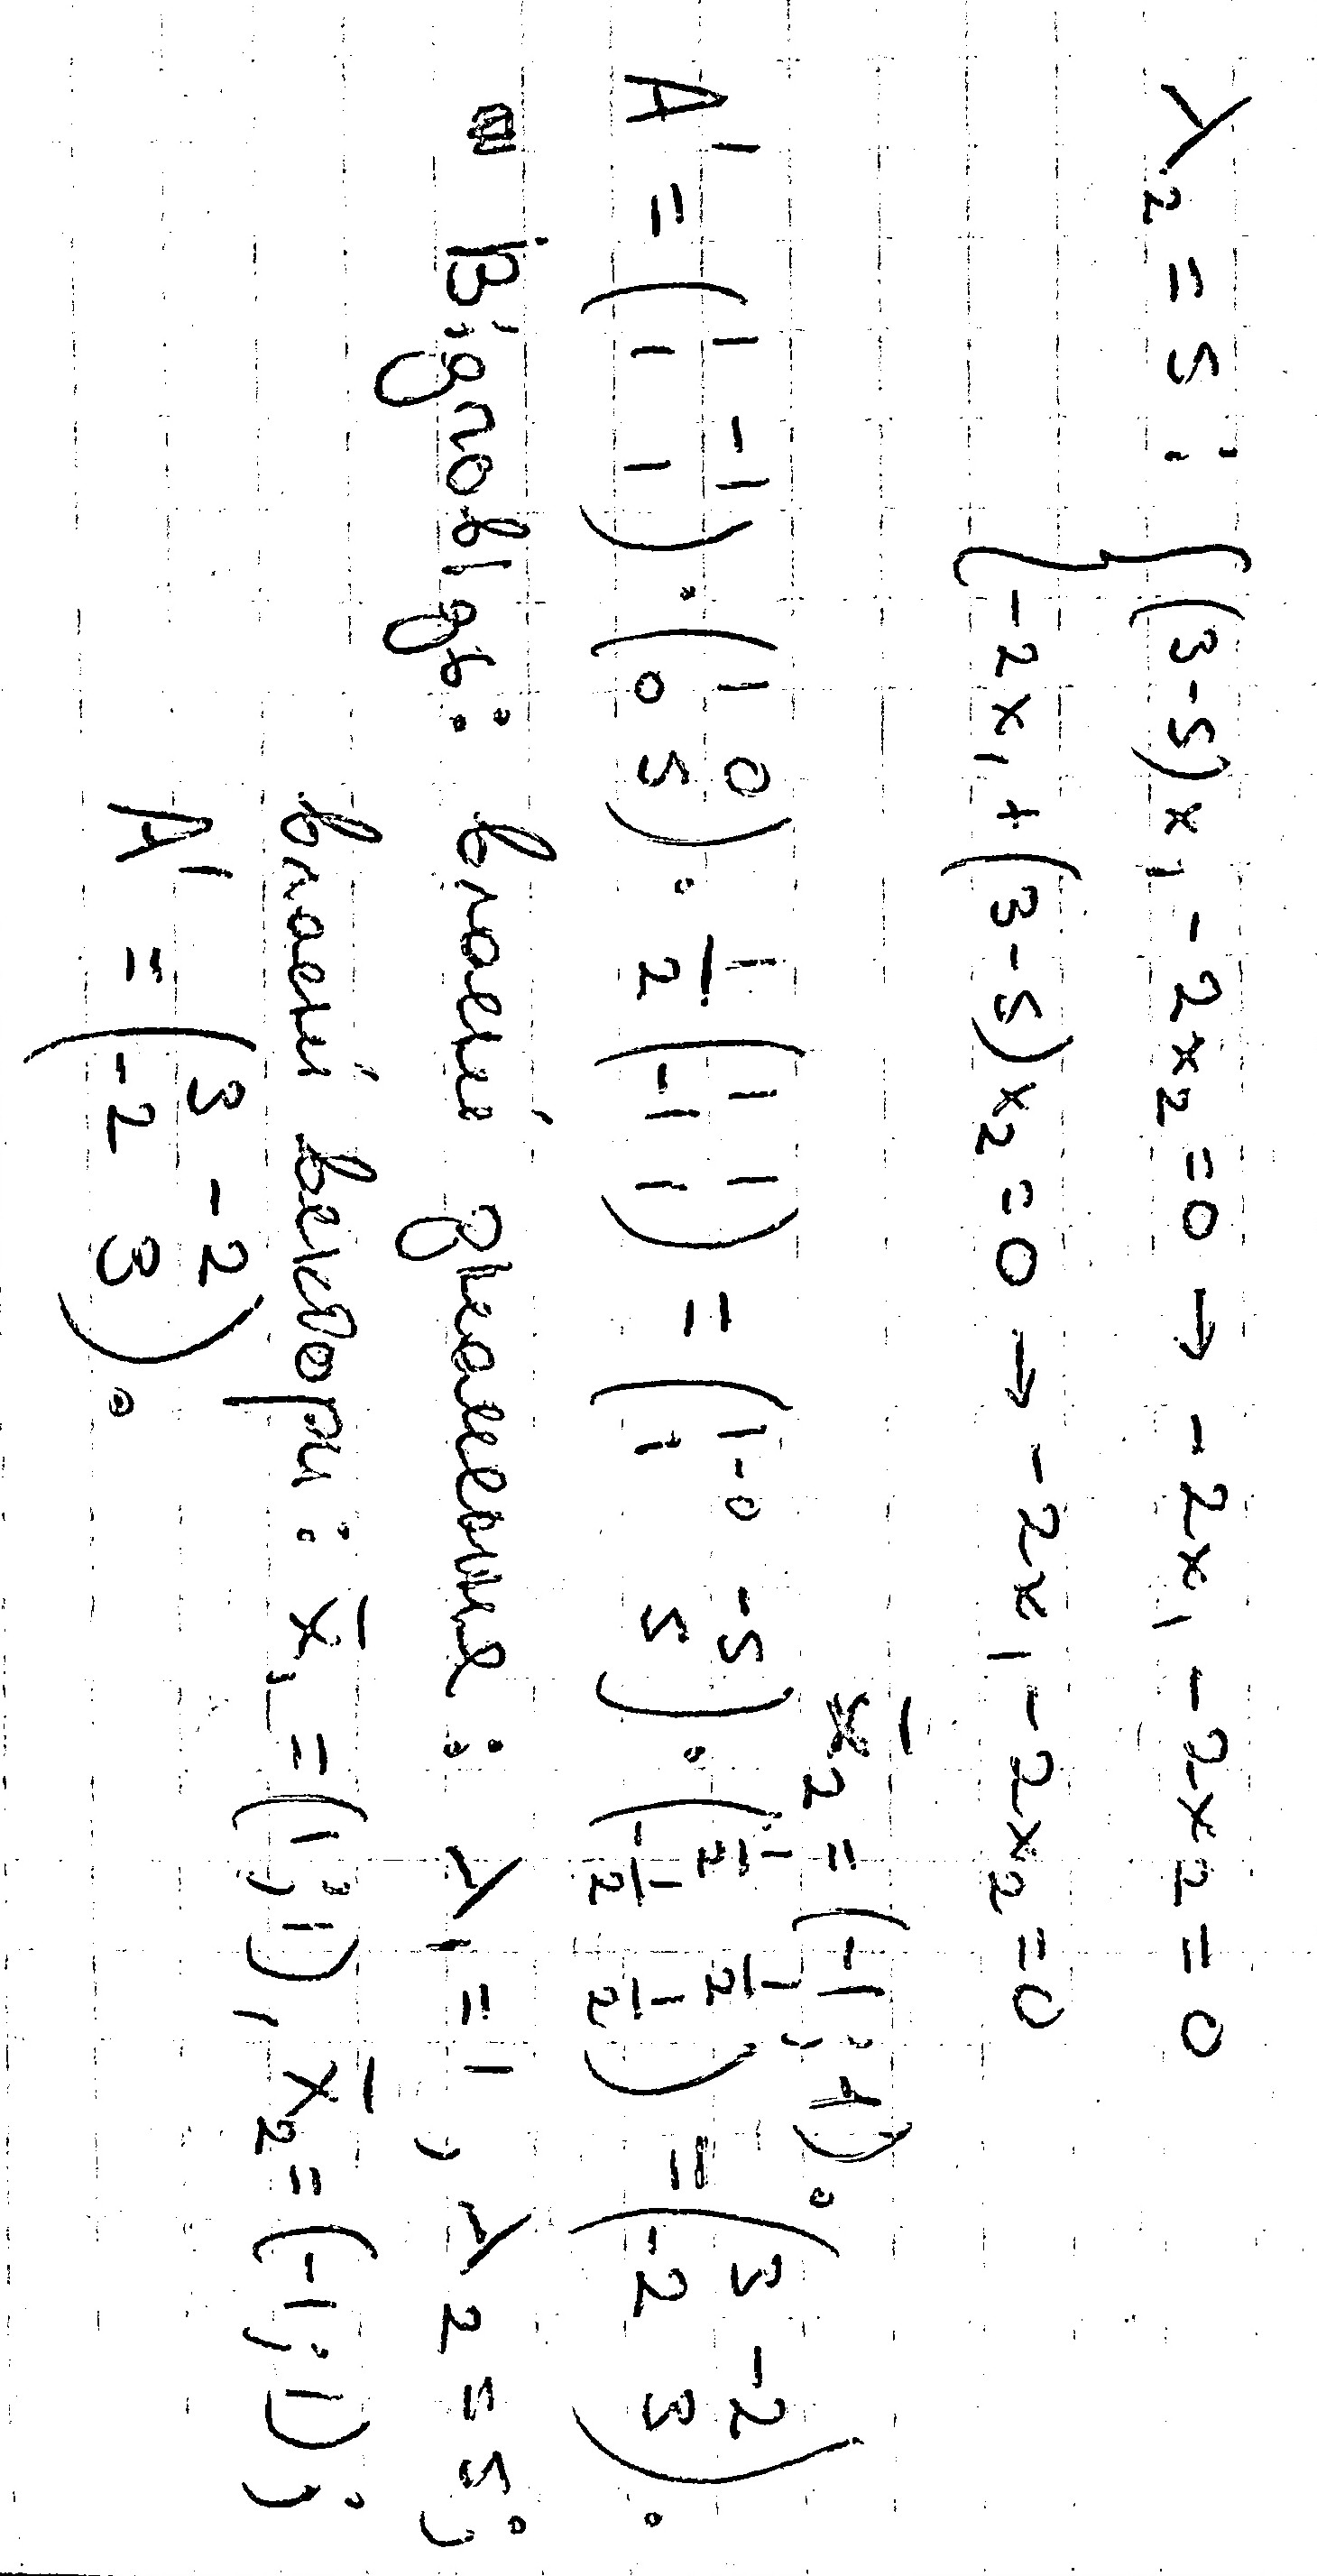
\includegraphics[width=10cm,angle=90]{ons/18.jpg}\\

\end{document}
